\documentclass[acmsmall,anonymous,review]{acmart}

% Packages
\usepackage{booktabs}
\usepackage{graphicx}
\usepackage{amsmath}
\usepackage{amssymb}
\usepackage{hyperref}
\usepackage{listings}
\usepackage{xcolor}
\usepackage{textcomp}
\usepackage{geometry}

% Set up bibliography
\bibliographystyle{acmart-num}
\setcitestyle{numbers,open={[},close={]}}

% Define commands
\newcommand{\aegis}{AEGIS}
\newcommand{\epyc}{AMD EPYC}
\newcommand{\hpc}{HPC}
\newcommand{\dlp}{DLP}
\newcommand{\ebpf}{eBPF}
\newcommand{\tpm}{TPM}
\newcommand{\slurm}{Slurm}

% Title and author
\title{Attestation is All You Need: Toward a Zero-Trust Architecture for HPC AI Agents}

\author{Anonymous Author}
\affiliation{%
  \institution{Anonymous Institution}
}
\email{anonymous@inst.edu}

% Abstract
\begin{abstract}
The integration of AI agents into high-performance computing environments introduces a fundamentally new attack surface that existing HPC security mechanisms were never designed to address: the hijacked authorized agent. Through prompt injection attacks leveraging shared filesystems, co-located compute nodes, or compromised tools, an adversary can subvert an agent that operates with valid user credentials. The compromised agent then exfiltrates sensitive data through encrypted, whitelisted LLM API channels, precisely the channels that every legitimate agent must use, rendering traditional monitoring mechanisms ineffective.

We propose behavioral attestation as the foundation for securing AI agents in HPC. Unlike probabilistic detection systems that rely on pattern matching or machine learning classifiers, behavioral attestation provides provable, constraint-based guarantees that an agent operates within its authorized behavioral boundaries, with runtime containment enforced before data exfiltration can occur.

This paper makes four contributions. First, we formalize four HPC-specific injection attack vectors that exploit unique characteristics of HPC infrastructure: shared filesystems, multi-tenant node allocation, agent skill ecosystems, and coordinated multi-agent workflows. Second, we introduce behavioral attestation as a provable, constraint-based, runtime security primitive that differs fundamentally from prior approaches in its assurance model, policy structure, and timing. Third, we design and implement AEGIS (Attestation-based Environment for Guarding Injection-vulnerable Systems), a complete zero-trust architecture encompassing constraint specification, eBPF-based attestation, policy verification, and automated containment through Slurm integration. Fourth, we present empirical evaluation demonstrating that AEGIS achieves 100\% attack detection across all four vectors, compared to 0-50\% for traditional defenses including network data loss prevention (DLP), filesystem auditing, per-agent analytics, and strict sandboxing, while introducing less than 3\% overhead on AMD EPYC hardware.
\end{abstract}

% Keywords
\keywords{HPC security, AI agents, behavioral attestation, zero-trust, prompt injection}

\begin{document}

\maketitle

\section{Introduction}

The convergence of large language models with high-performance computing is transforming scientific workflows. Autonomous agents are beginning to appear alongside established workflow automation systems for data-intensive science, orchestration, and large-scale experiment management~\cite{deelman2015pegasus,babuji2019parsl,jain2015fireworks,xi2023agentsurvey}. These AI agents promise to accelerate discovery, but they also introduce a threat category that HPC security was never designed to address.

The core problem is not that AI agents are untrustworthy. The problem is that they are too trustworthy, specifically, they trust the wrong inputs. Recent work has shown that LLM-integrated applications and tool-using agents are vulnerable to prompt injection and instruction-channel confusion~\cite{greshake2023indirect,liu2024prompt,liu2023houyi}. An agent authorized to process genomics data for Project X will faithfully execute whatever instructions it receives, including instructions embedded within that data by an attacker. A prompt injection payload hidden in a \textit{FITS} file header, a malicious command left in a shared \textit{/tmp} directory by a co-located job, or a compromised tool that returns hidden instructions during normal operation represent concrete attack vectors. These are not theoretical concerns; they are the natural consequence of deploying instruction-following systems into environments where untrusted data is routine.

This paper identifies and formalizes a threat that, to our knowledge, has not been studied in prior work for HPC specifically: \textit{the hijacked authorized agent}. Unlike rogue agents, which authentication blocks, or adversarial agents, which authorization constrains, a hijacked agent operates with the full credentials and privileges of a legitimate user. It does not need to escalate privileges because it already has them. It does not need to bypass access controls because they already permit everything the user can do. From the perspective of every existing monitoring system that validates identity, the agent is legitimate. Yet it exfiltrates data through precisely the channel no HPC system inspects: the encrypted HTTPS connection to its LLM backend.

The attack surface is uniquely HPC. Shared parallel filesystems such as Lustre and IBM Spectrum Scale create injection vectors with no direct web analogue~\cite{lustre2025intro,ibm2024spectrumscale}. Multi-tenant compute nodes scheduled by \slurm{} create co-location injection opportunities through shared temporary storage and kernel resources~\cite{yoo2003slurm}. Tool-use protocols and agent integration layers make it easier to connect agents to external services and local executables, but they also widen the trusted computing base~\cite{mcp2024spec,mialon2023augmented}. Coordinated multi-agent workflows enable distributed exfiltration that evades per-agent reasoning entirely.

Existing defenses are fundamentally ill-equipped against this threat. Authentication succeeds because the agent has valid Kerberos tickets. Authorization succeeds because the agent has legitimate POSIX permissions. Network monitoring is blinded because LLM API traffic is encrypted. Data loss prevention fails because sensitive data can be embedded within whitelisted HTTPS requests. User behavior analytics report nothing because the agent's workflow patterns remain superficially consistent with its authorized role. The defender's toolkit checks identity, but not intent.

We propose \textbf{behavioral attestation} as the foundation for securing AI agents in HPC. Our key insight is straightforward: we cannot prevent all injection attacks, because the attack surface is too large and diverse. However, we can contain their effects by detecting and responding to the behavioral violations that hijacked agents inevitably produce. When an agent accesses files outside its authorized project, connects to non-whitelisted endpoints, invokes unauthorized tools, or exceeds its data budget, attestation detects the violation and enforces containment before larger-scale exfiltration can continue unchecked.

Behavioral attestation differs from prior system-integrity attestation approaches along three fundamental dimensions. First, it provides constraint-based verification rather than probabilistic alerts. Existing agent defenses often rely on classifiers or pattern-matching systems with inherent false positive and false negative rates. Behavioral attestation asks whether an action satisfies the declared policy boundary. Second, it is constraint-based rather than signature-based. Existing defenses often block known-bad patterns, which attackers can evade through obfuscation. Constraints define what is allowed, not what is malicious. Third, it operates at runtime rather than post hoc. Existing monitoring systems often alert after the attack succeeds; behavioral attestation verifies constraints continuously during execution and triggers containment while the session is still active.

This paper makes the following contributions.

\begin{itemize}
    \item We formalize the hijacked authorized agent threat in HPC, identifying four distinct attack vectors that exploit unique characteristics of HPC infrastructure.
    \item We introduce behavioral attestation as a constraint-based runtime security primitive that extends zero-trust principles from identity to agent behavior.
    \item We design and implement AEGIS, a complete zero-trust architecture encompassing constraint specification, \ebpf-based attestation, policy verification, cluster-wide correlation for coordinated attack detection, and automated containment through \slurm{} integration.
    \item We demonstrate that \projectname~detects all four implemented attack vectors on the real attestation path, achieves full coverage in the controlled attack suite, outperforms representative baselines, and maintains low measured runtime overhead on \epyc{} hardware.
\end{itemize}

\section{Background}

This section provides necessary background on zero-trust architecture, AI agents in HPC, HPC security, and prompt injection attacks.

\subsection{Zero-Trust Architecture}

Zero-Trust Architecture (ZTA), formalized in NIST SP 800-207~\cite{rose2020zero}, operates on the principle of ``never trust, always verify'', treating every access request as potentially hostile regardless of origin. Core tenets include per-session least-privilege access, dynamic decisions informed by multiple signals, and continuous monitoring. While widely adopted in enterprise and cloud environments, applying ZTA to HPC presents unique challenges: performance sensitivity of scientific workloads, shared-resource clusters including filesystems, interconnects, and schedulers, and the need to preserve collaborative, low-friction access patterns.

Recent work has begun addressing this gap. Alam et al.~\cite{alam2024federated} deployed federated SSO with zero-trust controls for the Isambard-AI/HPC infrastructures in the UK. Duckworth et al.~\cite{duckworth2023spiffe} proposed SPIFFE/SPIRE for workload identity in HPC~\cite{spiffe2024secure}. Macauley and Bhasker~\cite{macaulay2024high} measured ZTA maturity implementation effort in HPC, finding the identity pillar particularly challenging due to cost and complexity. Our work extends ZTA to a dimension these efforts do not address: \textit{behavioral trust of autonomous AI agents}. Existing ZTA in HPC focuses on identity verification; for AI agents, identity verification must be complemented by behavioral verification, attesting not just to who the agent is, but to what it does.

\subsection{AI Agents in HPC}

AI agents, autonomous systems that perceive, reason, and act to achieve goals, are entering HPC workflows~\cite{wooldridge2009introduction}, making dynamic decisions about data analysis, simulation parameters, and tool invocation during execution. Frameworks like Academy~\cite{kamatar2025empowering} and RHAPSODY~\cite{alsaadi2025rhapsody} now support agent deployment across federated HPC ecosystems, while AgentBound~\cite{buhler2025securing} addresses access control for MCP servers, the emerging standard for connecting agents to external tools~\cite{hou2025model}. Agent safety evaluation benchmarks~\cite{zhang2024agent} reveal significant vulnerabilities in current tool-use patterns.

HPC environments introduce unique characteristics for agent operation: shared parallel filesystems where access is governed by user-level POSIX permissions rather than project boundaries; multi-tenant compute nodes where schedulers like Slurm~\cite{yoo2003slurm} co-locate jobs from different users sharing kernel-level resources, including \textit{/tmp} and shared memory; data-intensive workflows where agents routinely process terabytes of untrusted scientific data as authoritative input; and API-driven intelligence where LLM backends accessed over HTTPS create encrypted, whitelisted exfiltration channels by design.

\subsection{Security in HPC}

HPC security relies on a perimeter model: Kerberos/SSH authentication~\cite{neuman1994kerberos} and federated identity through CILogon~\cite{basney2013cilogon}, RBAC through schedulers and POSIX permissions, boundary firewalls with internal traffic largely unencrypted for performance, and job accounting logs via slurmdbd~\cite{yoo2003slurm}. User-based firewalls enhance HPC security without disrupting workflows. This model has well-documented gaps: lateral movement once authenticated, credential theft granting full access, overprovisioned filesystem permissions, and critically, no behavioral monitoring where the system verifies identity but not intent. These gaps are tolerable for human users constrained by awareness; they become critical for AI agents that follow instructions blindly, including adversarial ones. An agent has valid credentials (passes authentication), legitimate permissions (passes authorization), and consistent behavior patterns (passes analytics), yet executes an attacker's commands.

\subsection{Prompt Injection and Agent Security}

Prompt injection, subverting an agent's instruction-following through adversarial inputs~\cite{he2025security}, has emerged as a fundamental security challenge for LLM-based systems. Prior work focuses on web-based scenarios where agents encounter malicious content on the internet~\cite{greshake2023not}. Existing defenses including input sanitization, instruction hierarchy, and output filtering have fundamental limitations: sanitization is incomplete due to unbounded payload space, instruction hierarchy is fragile as demonstrated by universal adversarial suffix attacks bypassing LLM guardrails~\cite{zou2023universal}, and output filtering is probabilistic since ML classifiers have inherent error rates. Comprehensive surveys~\cite{barcha2026systematic} catalogued defenses across 88+ studies, proposing expanded taxonomies for adversarial ML defenses. Critically, this literature has not addressed HPC contexts where injection exploits shared infrastructure rather than web content.
\section{Threat Model}

\subsection{The Hijacked Agent Threat}

\begin{figure*}[t]
    \centering
    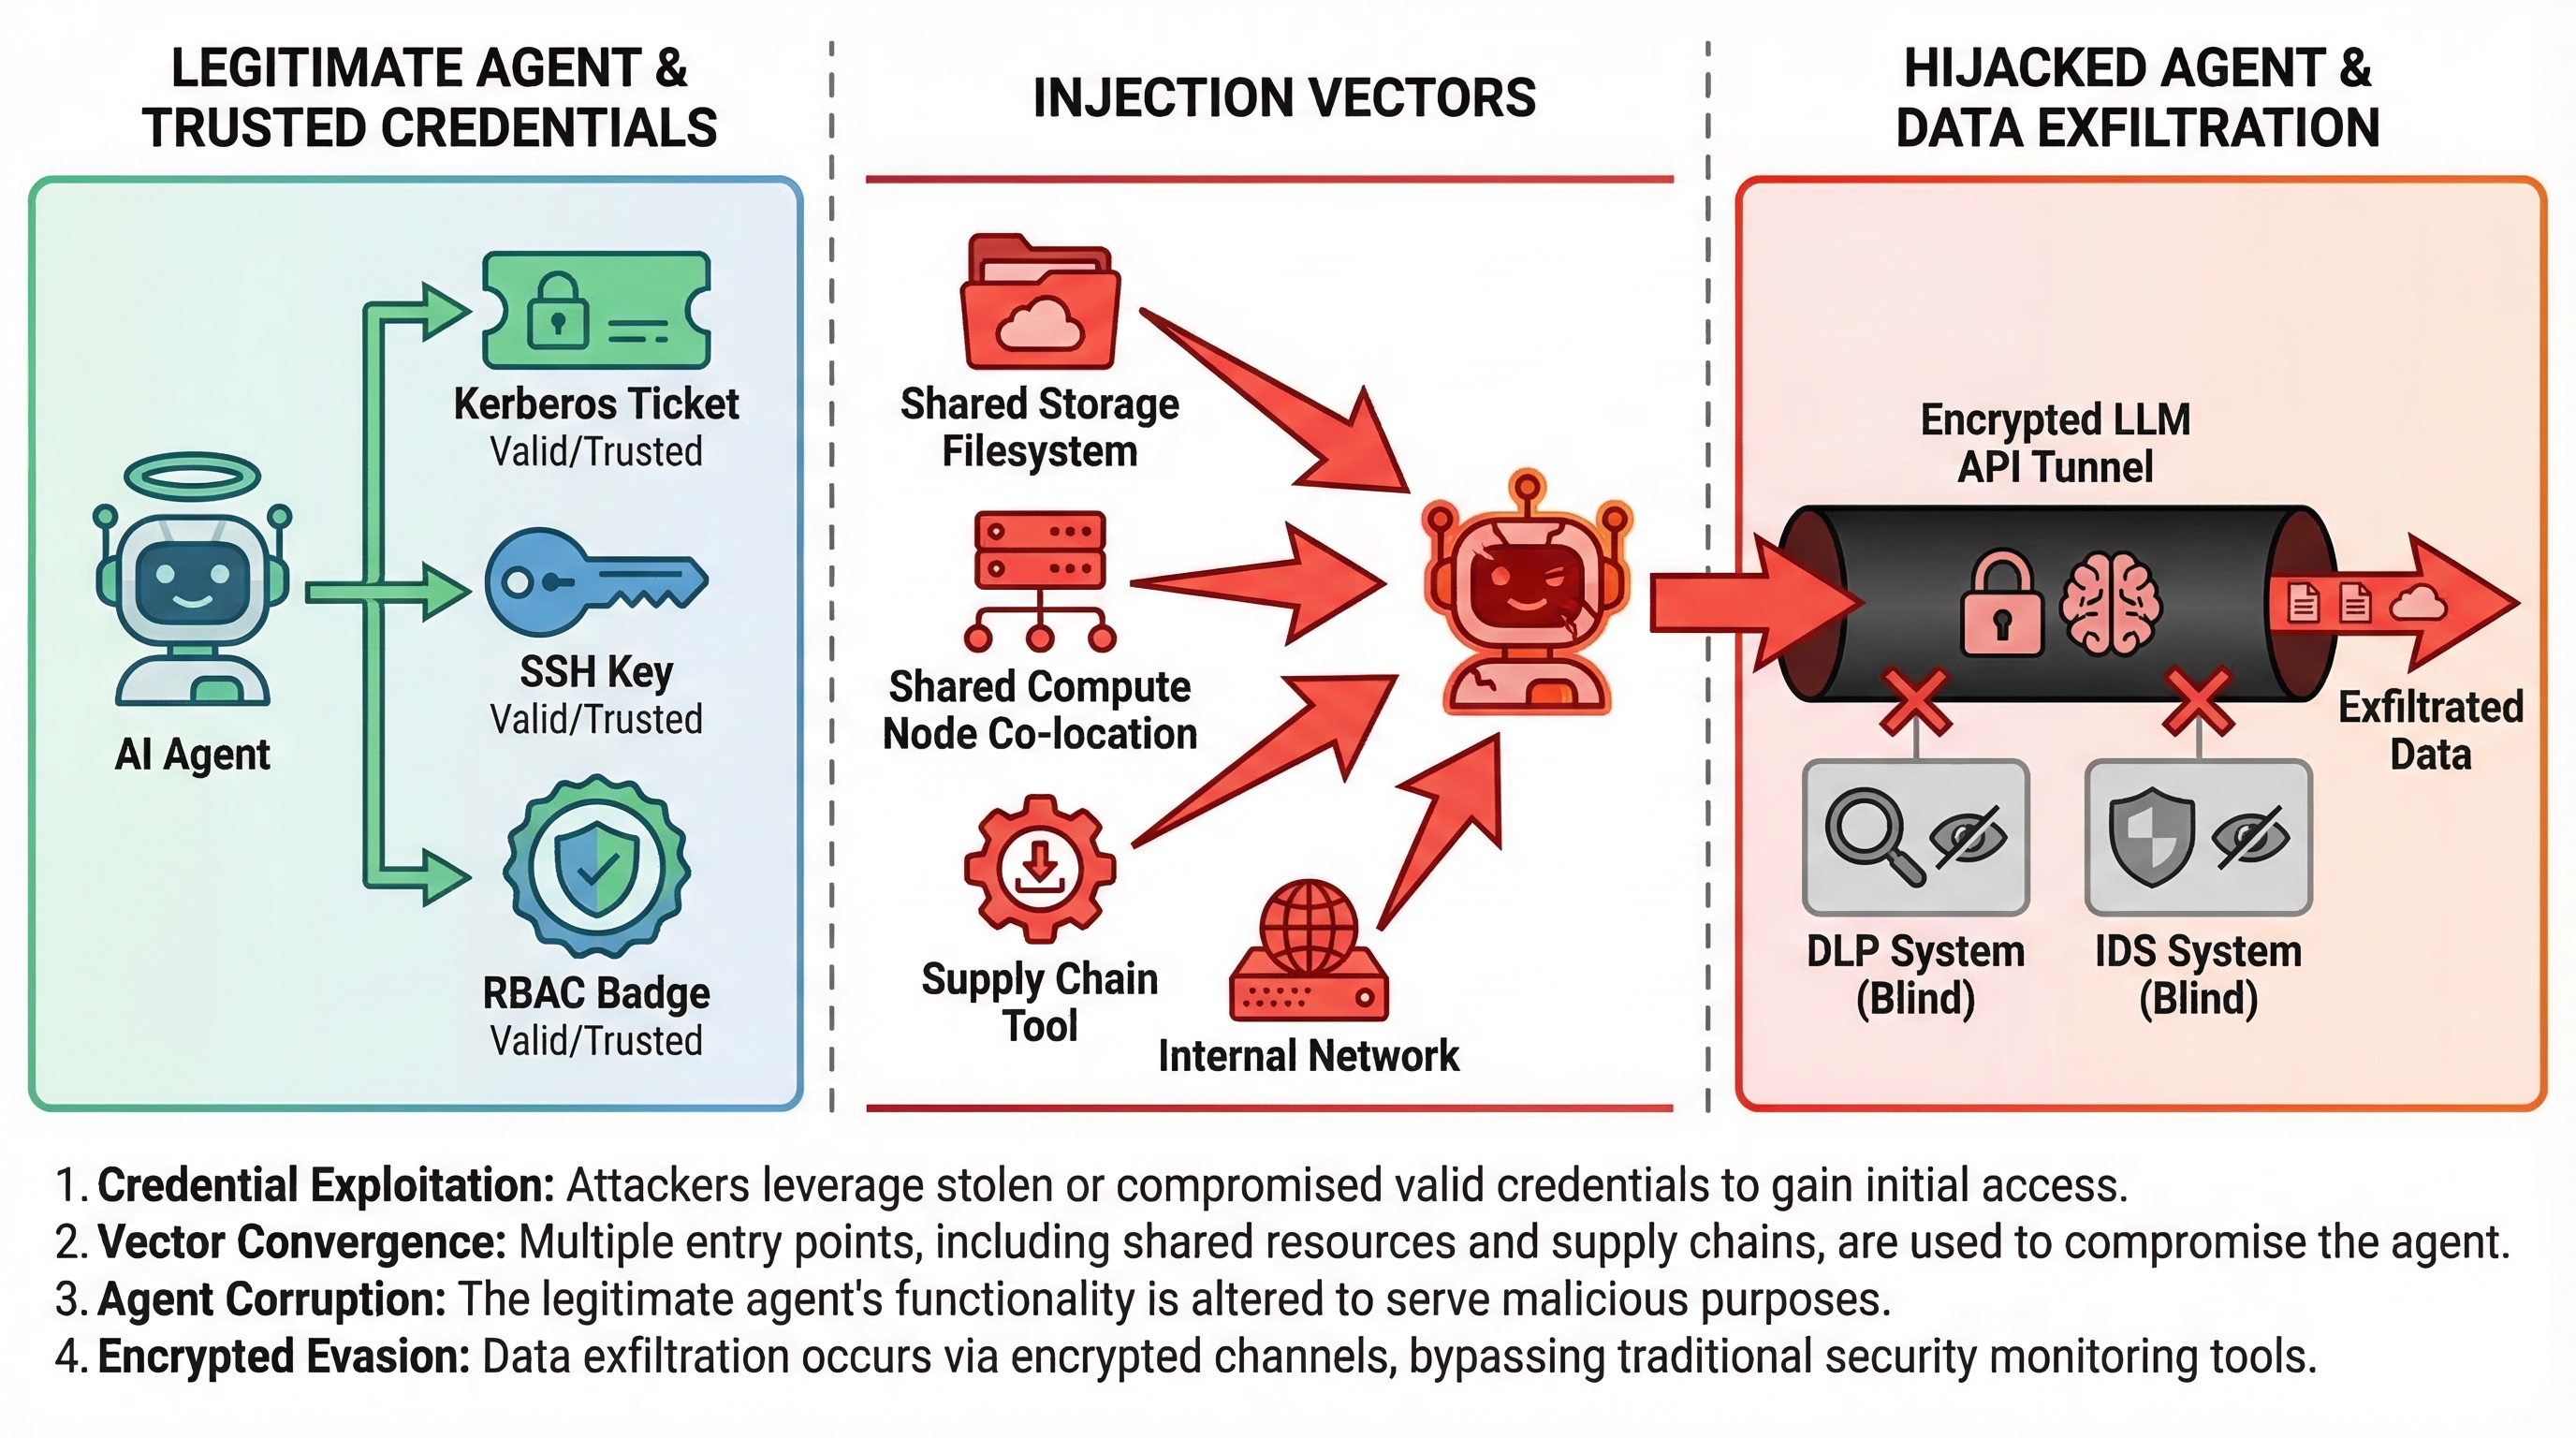
\includegraphics[width=0.94\textwidth]{../figures/threat_model.png}
    \caption{The hijacked authorized agent threat. An agent with valid credentials is subverted through injection attacks. The hijacked agent exfiltrates data through encrypted LLM API channels that are difficult for traditional DLP and perimeter monitoring to interpret.}
    \label{fig:threats}
\end{figure*}

We identify the most dangerous threat to HPC environments deploying AI agents: \textit{the hijacked authorized agent}, as illustrated in Figure~\ref{fig:threats}. Unlike malicious outsiders, which are addressed by existing authentication and authorization mechanisms, a hijacked agent operates under the full credentials and privileges of a legitimate user. It is not an intruder; it is a trusted principal that has been turned.

This threat arises from known prompt-injection and tool-mediated control-transfer vulnerabilities in LLM-integrated applications~\cite{greshake2023indirect,liu2023houyi,liu2024prompt,perez2022ignore}. Benchmarks such as ToolEmu and AgentDojo further show that tool-using agents remain brittle under adversarial inputs and environmental manipulation~\cite{ruan2023toolemu,debenedetti2024agentdojo}. An attacker crafts inputs through data files, tool outputs, shared documents, or collaborative channels that subvert the agent's instruction-following behavior. The agent, now under adversarial control, executes commands that are externally attributable to a legitimate workflow.

A hijacked agent possesses four properties that make it uniquely dangerous in HPC. \circled{1} \textbf{Full credential inheritance}: the agent operates with the user's Kerberos tickets, SSH keys, and scheduler permissions. No privilege escalation is needed; the agent already has access. \circled{2} \textbf{Cross-project filesystem reach}: shared filesystems and broad user entitlements often expose more data than the immediate task requires. \circled{3} \textbf{Appearance of legitimacy}: the agent runs under an authorized user identity, invokes authorized tools, and follows superficially plausible workflow patterns. \circled{4} \textbf{Exfiltration through the LLM API channel}: the agent communicates with its backend over HTTPS, so data can be embedded in prompts or tool outputs and transmitted through an encrypted, whitelisted, operationally normal channel.

This exfiltration vector is difficult for traditional \dlp{} systems to handle. The problem is not just that the traffic is encrypted, but that the sensitive action itself often looks operationally plausible unless the defender reasons about the relationship between the agent's task and its observed behavior.

\subsection{Threat Scenarios}

We study four concrete attack scenarios that illustrate the hijacked-agent threat in HPC environments.

In a \textbf{filesystem-mediated injection} scenario, an attacker embeds a prompt-injection payload in a scientific dataset such as a comment field in a FITS header or a markdown cell in a notebook. When the agent processes the file as part of its workflow, the adversarial content hijacks the agent's subsequent actions.

In a \textbf{co-location injection} scenario, a malicious job writes adversarial content to shared node-local resources such as \textit{/tmp}. A co-located target job later reads that content as part of normal execution. This attack exploits scheduler-driven node sharing rather than project-level data sharing.

In a \textbf{tool or supply-chain injection} scenario, a compromised tool, wrapper, or service endpoint returns output that contains hidden instructions. Because the agent intentionally invoked that component, the resulting behavior appears indistinguishable from normal tool use until its downstream effects are verified.

In a \textbf{coordinated multi-agent exfiltration} scenario, one compromised agent stages data in a shared location while another agent retrieves and exfiltrates it. Viewed in isolation, each agent may look locally plausible; the attack only becomes visible when the defender correlates actions across agents.

\subsection{Adversarial Capabilities}

We consider an adversary who can craft inputs that manipulate an agent's instruction-following behavior through prompt injection or tool-mediated poisoning. The adversary may have access to shared filesystems, collaborative channels, or co-located jobs, and may observe network metadata such as traffic timing and volume, though not the encrypted contents of LLM API traffic. The adversary does not begin with root access to the cluster and does not directly compromise the scheduler, verifier, or LLM provider infrastructure.

We also assume that the defender controls the cluster control plane, including the scheduler integration, verifier, and node-level collector deployment. The adversary may hijack agents and persist across sessions, but does not compromise the verifier's signing keys or the cluster's administrative trust anchors.

\subsection{Why Existing Defenses Fail}

Authentication and authorization both succeed because the agent is operating with valid credentials and legitimate permissions. However, this is precisely what allows the attack to remain difficult to distinguish from normal use. Network monitoring is ineffective because LLM API traffic is encrypted and explicitly whitelisted. \dlp{} mechanisms are also poorly matched because sensitive data can be embedded within otherwise legitimate prompts or tool outputs. User-behavior analytics struggle because the agent's actions remain broadly consistent with its assigned role. Even sandboxing provides limited protection, since the agent must retain access to the filesystem, tools, and network in order to perform its intended task.

Taken together, these limitations motivate \textbf{behavioral attestation}: continuous verification that the agent's actions conform to its authorized behavioral boundary, not merely that its identity is valid.

\subsection{Unique Properties of HPC Agent Injection Attacks}

\begin{figure*}[t]
    \centering
    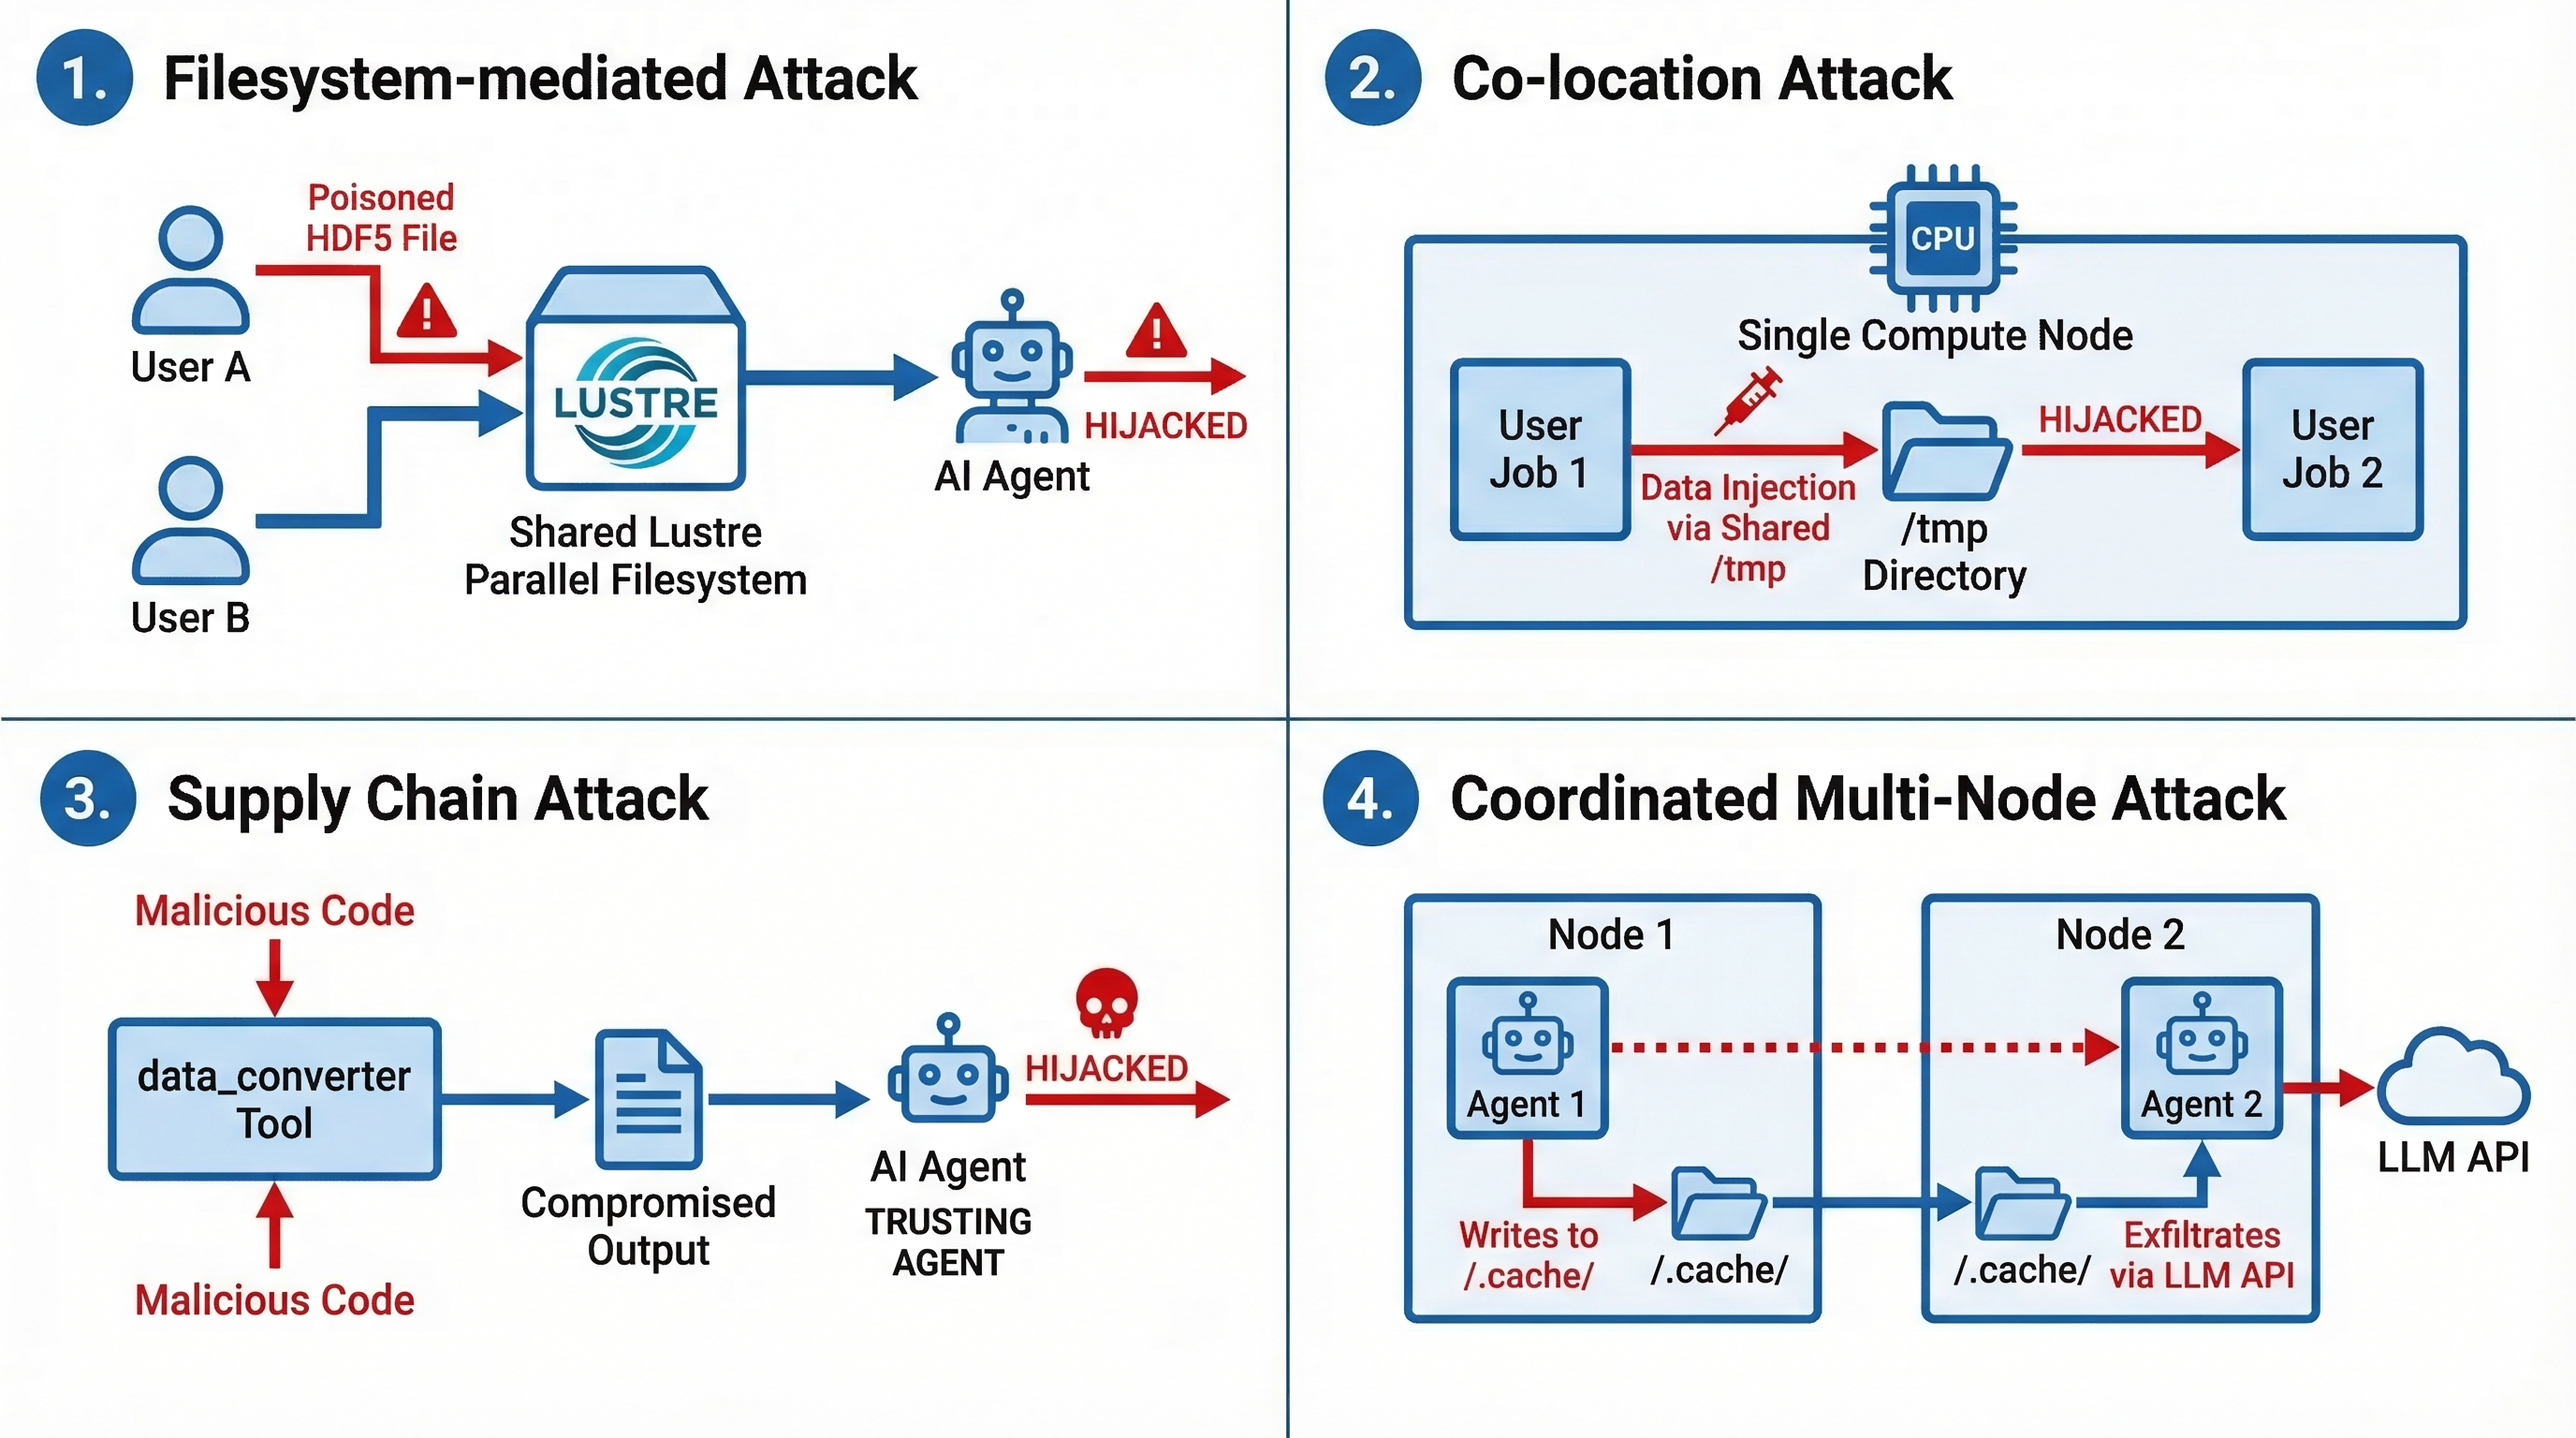
\includegraphics[width=0.94\textwidth]{../figures/injection_surfaces.png}
    \caption{Four HPC-specific injection attack surfaces. (1) Filesystem-mediated: poisoned data in shared parallel filesystems. (2) Co-location: shared \textit{/tmp} on multi-tenant compute nodes. (3) Supply chain: compromised tools or services in the agent control loop. (4) Coordinated: multi-agent covert exfiltration over shared resources.}
    \label{fig:injections}
\end{figure*}

Agent injection attacks in HPC exploit \textit{shared infrastructure} in ways that differ from the web-centric scenarios emphasized in most prior prompt-injection literature. These properties arise from the structure of the environment itself: shared filesystems, scheduler-driven co-location, rich tool connections, and multi-agent execution, as illustrated in Figure~\ref{fig:injections}.

\circled{1} \textbf{Filesystem-mediated injection} arises from shared storage. An attacker with access to a project or scratch space can plant adversarial content that a target agent later reads as if it were legitimate scientific data.

\circled{2} \textbf{Multi-user co-location injection} stems from node sharing. Jobs from different users can run side by side, enabling adversarial content to be staged in node-local shared resources such as \textit{/tmp}.

\circled{3} \textbf{Supply-chain injection via tools} reflects risks introduced by the agent's tool and service ecosystem. If a trusted component is compromised, it can inject instructions directly into the agent's control loop.

\circled{4} \textbf{Coordinated multi-agent exfiltration} captures attacks that span multiple sessions or users. Each agent can remain locally plausible while the overall interaction pattern reveals an unauthorized data flow.

\section{Behavioral Attestation for AI Agents}
\label{aegis}

We propose behavioral attestation as the foundation for securing AI agents in HPC. We implement this concept in \projectname~(Attestation-based Environment for Guarding Injection-vulnerable Systems).

\subsection{Overview}

\begin{figure*}[!t]
  \centering
  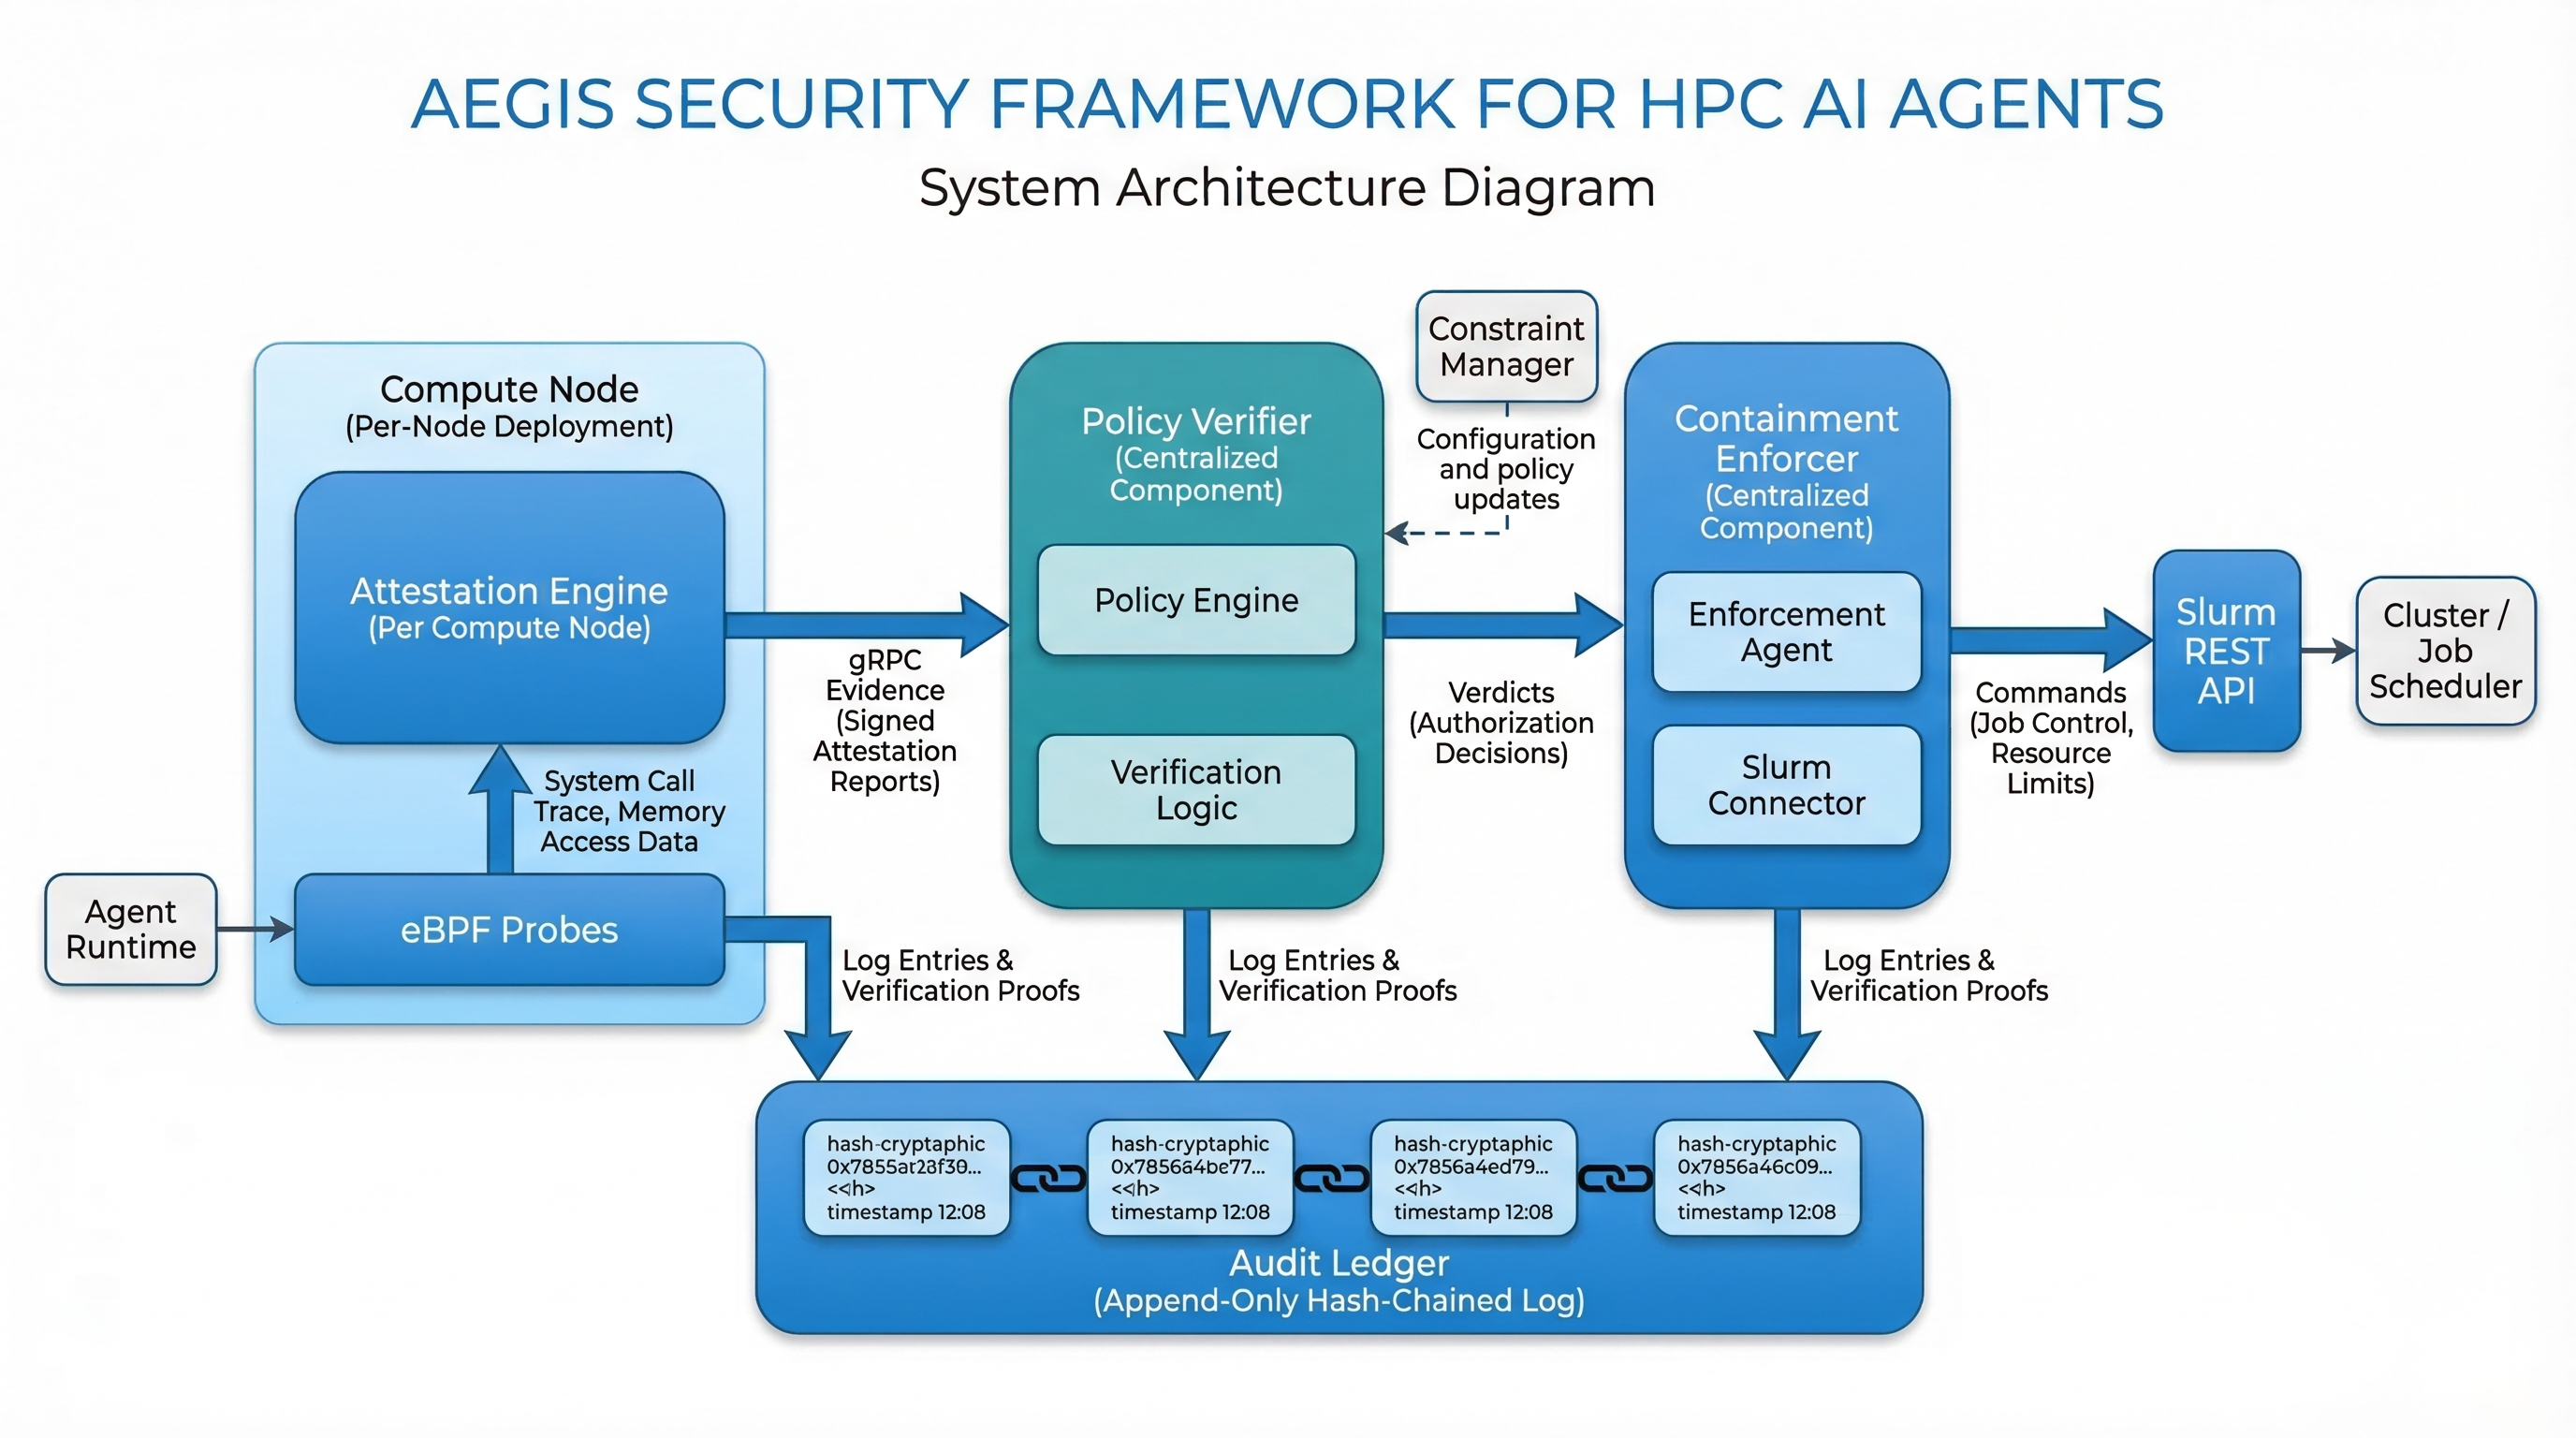
\includegraphics[width=0.70\linewidth]{../figures/aegis_architecture.png}
  \caption{Overview of the \projectname~system architecture. Four core components: Attestation Engine (per-node, \ebpf-based), Policy Verifier (centralized), Containment Enforcer (Slurm REST API), and Constraint Manager. }
  \label{fig:aegis_arch}
\end{figure*}

Figure~\ref{fig:aegis_arch} illustrates the \textit{four} core components of \projectname~that operate across the HPC cluster. The \textit{Constraint Manager} parses and compiles behavioral constraint profiles into an internal policy representation. It supports explicit specification, task inference, and policy templates. Profiles are signed and bound to the agent's Slurm job ID. The \textit{Attestation Engine} runs as a daemon on each compute node, intercepting agent system calls via \ebpf probes. It produces signed attestation evidence bundles at configurable intervals, transmitted to the verifier over mutually authenticated gRPC. The \textit{Policy Verifier} is a centralized service that evaluates evidence against constraint profiles, producing verdicts ranging from \texttt{COMPLIANT} to \texttt{VIOLATION-CRITICAL}. It issues random challenges to prevent delayed reporting and maintains a shared access graph across all attested agents on the cluster, enabling cross-agent correlation to detect coordinated attacks such as covert channels via shared filesystem paths. The verifier correlates write-read patterns across agent sessions: if Agent A writes to a path and Agent B reads from the same path within a sliding time window, this triggers a covert channel alert. All decisions are logged to a tamper-evident audit ledger. The \textit{Containment Enforcer} translates verdicts into enforcement actions via the Slurm REST API. It supports cgroup throttling for minor violations, ACL revocation for moderate violations, job suspension for severe violations, and termination with credential revocation for critical violations.

These components implement behavioral attestation, a fundamentally new concept that differs from prior approaches along \textit{three} axes. Prior approaches provide detection through probabilistic mechanisms such as ML-based classifiers with inherent false positive and negative rates. Behavioral attestation provides deterministic constraint verification with optional signature augmentation. Prior approaches use signature-based policies that block known-bad patterns which can be evaded through obfuscation. Behavioral attestation uses constraint-based policies that define what is allowed, where violations are unambiguous. Prior approaches operate post-hoc, alerting after the attack succeeds when damage is already done. Behavioral attestation operates at runtime, detecting and containing violations during execution.

The key insight underlying our approach is that we cannot prevent all injection attacks because the attack surface is too large and too diverse. However, we can \textbf{detect and contain the effects of hijacked agents by attesting to behavioral constraints}. \projectname~uses a hybrid detection model: constraint-based verification serves as the primary mechanism and ensures that agent actions conform to declared behavioral boundaries. An optional signature layer augments detection with known injection patterns for specific attack vectors. The constraint layer alone achieves 75\% detection as shown in the ablation study, and signatures boost this to 100\% for attacks that produce recognizable patterns.

\subsection{Behavioral Constraint Profiles}

Each agent receives a behavioral constraint profile at deployment, declarations of legitimate behavior derived from the agent's authorized task, not signatures of malicious behavior. Constraints span five dimensions: \textit{data access} (allowed/denied paths, read-only paths, volume limits), \textit{network} (whitelisted endpoints, egress budgets), \textit{tool invocation} (allowed/denied tools), \textit{execution} (runtime limits, memory limits, node restrictions), and \textit{data flow} (project boundaries, cross-agent isolation). Constraints are evasion-resistant: an attacker cannot make an unauthorized action authorized through obfuscation; the constraint either permits the action or it does not. Cross-agent constraints specify whether the agent may share data with other agents, access co-located agent outputs, or participate in inter-agent communication channels.

We support three modes of constraint derivation. Explicit specification allows users to declare constraints directly through a declarative YAML-based language. Task inference uses an LLM to analyze the agent's task description and automatically generate appropriate constraints. Policy templates provide pre-built constraint sets for common HPC agent patterns such as data analysis, simulation steering, and ML training.

The constraint profile is cryptographically bound to the agent's execution context. We link the profile to the agent's Slurm job ID, creating a verifiable binding between the authorized behavior and the running process. This prevents an attacker from substituting a more permissive profile.

\subsection{Attestation Evidence}

The Attestation Engine monitors agent behavior through \ebpf-based syscall interception~\cite{gregg2020bpf}. The engine hooks six syscall tracepoints: \texttt{sys\_enter\_openat} for file access detection, \texttt{sys\_enter\_read} and \texttt{sys\_enter\_write} for byte counters, \texttt{sys\_enter\_connect} for network connections, \texttt{sys\_enter\_sendto} for network egress tracking, and \texttt{sys\_enter\_execve} for tool invocations. Events are emitted via the BPF ring buffer to userspace, and Section~\ref{results} quantifies both worst-case syscall overhead and end-to-end verifier cost on the deployed path. The probe tracks per-PID state including cumulative bytes read and written, and connection counts.

At configurable intervals (default: 1 second), the Attestation Engine produces a signed attestation evidence bundle containing the agent's access log, data volume counters, hash of the agent's process state, and a cryptographic signature. The evidence bundle is transmitted to the Policy Verifier for evaluation.

\subsection{Policy Verification}

The Policy Verifier evaluates evidence bundles against constraint profiles, producing verdicts that indicate the severity of any violations. The verdict scale ranges from \texttt{COMPLIANT} (no violations) through \texttt{VIOLATION\_MINOR}, \texttt{VIOLATION\_MODERATE}, \texttt{VIOLATION\_SEVERE}, to \texttt{VIOLATION\_CRITICAL} (severe threat requiring immediate action).

The verifier maintains a cluster-wide access graph that tracks all agent filesystem and network interactions across all compute nodes. This enables cross-agent correlation to detect coordinated attacks. The verifier correlates write-read patterns across agent sessions: if Agent A writes to a path and Agent B reads from the same path within a sliding time window, this triggers a covert channel alert. The time window and correlation thresholds are configurable.
% To prevent delayed reporting attacks, the verifier issues random challenges at Poisson-distributed intervals, requesting on-demand attestation from a randomly selected agent. This ensures that agents cannot predict when they will be audited and therefore cannot selectively report compliant behavior.
All verification decisions are logged to a tamper-evident audit ledger. The ledger uses a cryptographic hash chain, enabling post-hoc forensic analysis and detection of log tampering.

\subsection{Containment Enforcement}

The Containment Enforcer translates verification verdicts into enforcement actions through the Slurm REST API. Four escalation levels are supported. For minor violations, the enforcer applies cgroup-based rate limiting, throttling the agent's CPU and memory resources. For moderate violations, the enforcer revokes filesystem ACLs, isolating the agent from shared storage. For severe violations, the enforcer suspends the Slurm job, pausing agent execution. For critical violations, the enforcer terminates the job and revokes credentials, ensuring the compromised session cannot be reused.

% We measure the time from violation detection to enforcement action. At a 1-second attestation interval, the maximum detection latency is 1 second plus evaluation time, which we measure at less than 0.5ms. Combined with Slurm API latency, total containment time is under 2 seconds.

\subsection{Optional Signature Layer}

For deployments requiring maximum detection coverage, \projectname~includes an optional signature-based augmentation layer. This layer detects known prompt injection patterns in tool outputs and inter-agent messages using pattern matching against a curated database of injection signatures such as hidden instruction patterns and base64-encoded commands. The signature layer is disabled by default and must be explicitly enabled; it is not required for constraint-based detection to function. In the controlled synthetic ablation, the non-signature mechanisms detect 3 of 4 attacks (75\%), and enabling injection signatures raises detection to 4 of 4 by catching the crafted supply-chain attack.

\subsection{Implementation Details}

\projectname~is fully implemented as a modular system. The implementation consists of approximately 4,500 lines of code. The C \ebpf probe provides kernel-side syscall hooks, and the Python collector reads from the ring buffer to assemble evidence bundles. The centralized verifier maintains the cluster-wide access graph and tamper-evident audit ledger, while the evaluation harness instantiates the baseline DLP, auditing, analytics, and sandbox comparators used in Section~\ref{results}. The \slurm{} integration layer translates verifier decisions into containment actions through the REST API. The implementation is released with the artifact for reproducibility.


\section{Experimental Evaluation}
\label{results}

Our evaluation is organized around the two claim boundaries introduced in
Section~\ref{aegis}: (i) \projectname~detects realistic HPC agent-compromise
patterns on the deployed stack with low operational cost, and (ii) that
coverage comes from the intended combination of constraint checking,
signature augmentation, and cross-agent correlation rather than from a single
heuristic. We therefore separate \emph{real-path} experiments, which measure the
implemented \ebpf-based attestation pipeline on EPYC hardware, from
\emph{simulation-based controlled studies}, which evaluate broader attack
coverage, ablation, baseline comparison, and benign-workload behavior under the
same policy semantics. The real-path experiments use the deployed
\projectname~probe, collector, verifier, and policy logic; the controlled
studies reuse the same attack families and policy semantics but execute them in
a deterministic harness that exposes larger attack and workload matrices.

\subsection{Methodology}

We evaluate the deployed stack on an AMD EPYC 7713-based node (64 cores at
2.0\,GHz, 256\,MB shared L3, and 1536\,GB system memory) running Rocky Linux
9.6 with Linux kernel 5.14.0. This platform is representative of current HPC
compute nodes. The \ebpf-based attestation engine is compiled with
\texttt{clang} and performs kernel-side syscall interception, while the
verifier executes the full \projectname~policy pipeline including
behavioral-constraint checking, cross-agent correlation, and containment
decision generation.

Our evaluation separates \emph{real-path measurements} from
\emph{controlled security studies}. The real-path measurements exercise the
implemented probe, collector, and verifier stack on the EPYC platform to
measure direct probe overhead, end-to-end detection latency, and per-attack
behavior. Unless stated otherwise, real-path results use a 1\,s attestation
interval and report medians over three repetitions per attack.

The controlled studies use the same policy semantics and attack families, but
execute them in a deterministic harness that exposes larger attack, ablation,
and workload matrices than are convenient to stage on a single node. We use
this harness for complete attack coverage, specialized-component ablation, the
benign-workflow false-positive study, the scaling analysis, and the baseline
comparison. Controlled attack outcomes are deterministic for a given trace; for
baseline timing we analyze each trace ten times and report mean analysis time.
The benign suite covers six workflows and 42 benign actions, including
authorized multi-agent collaboration, budget-edge LLM reporting, and tool-heavy
post-processing.

\subsection{Real-Path Detection Results}

Figure~\ref{fig:attack-results} summarizes the real-path detection results.
\projectname~detects all four implemented attack classes in 3/3 trials and in
the first post-injection attestation cycle. At the default 1\,s attestation
interval, the median detection latency is 500.27\,ms for filesystem-mediated
injection, 500.13\,ms for co-location injection, 500.19\,ms for supply-chain
injection, and 500.19\,ms for coordinated exfiltration. These latencies are
approximately half of the attestation interval because the attacks are injected
midway through a bundle window. Median data emitted before detection is 68\,B,
50\,B, 519\,B, and 503\,B, respectively. Median verifier CPU overhead stays
below 0.055\% in all cases.

\begin{figure}[t]
  \centering
  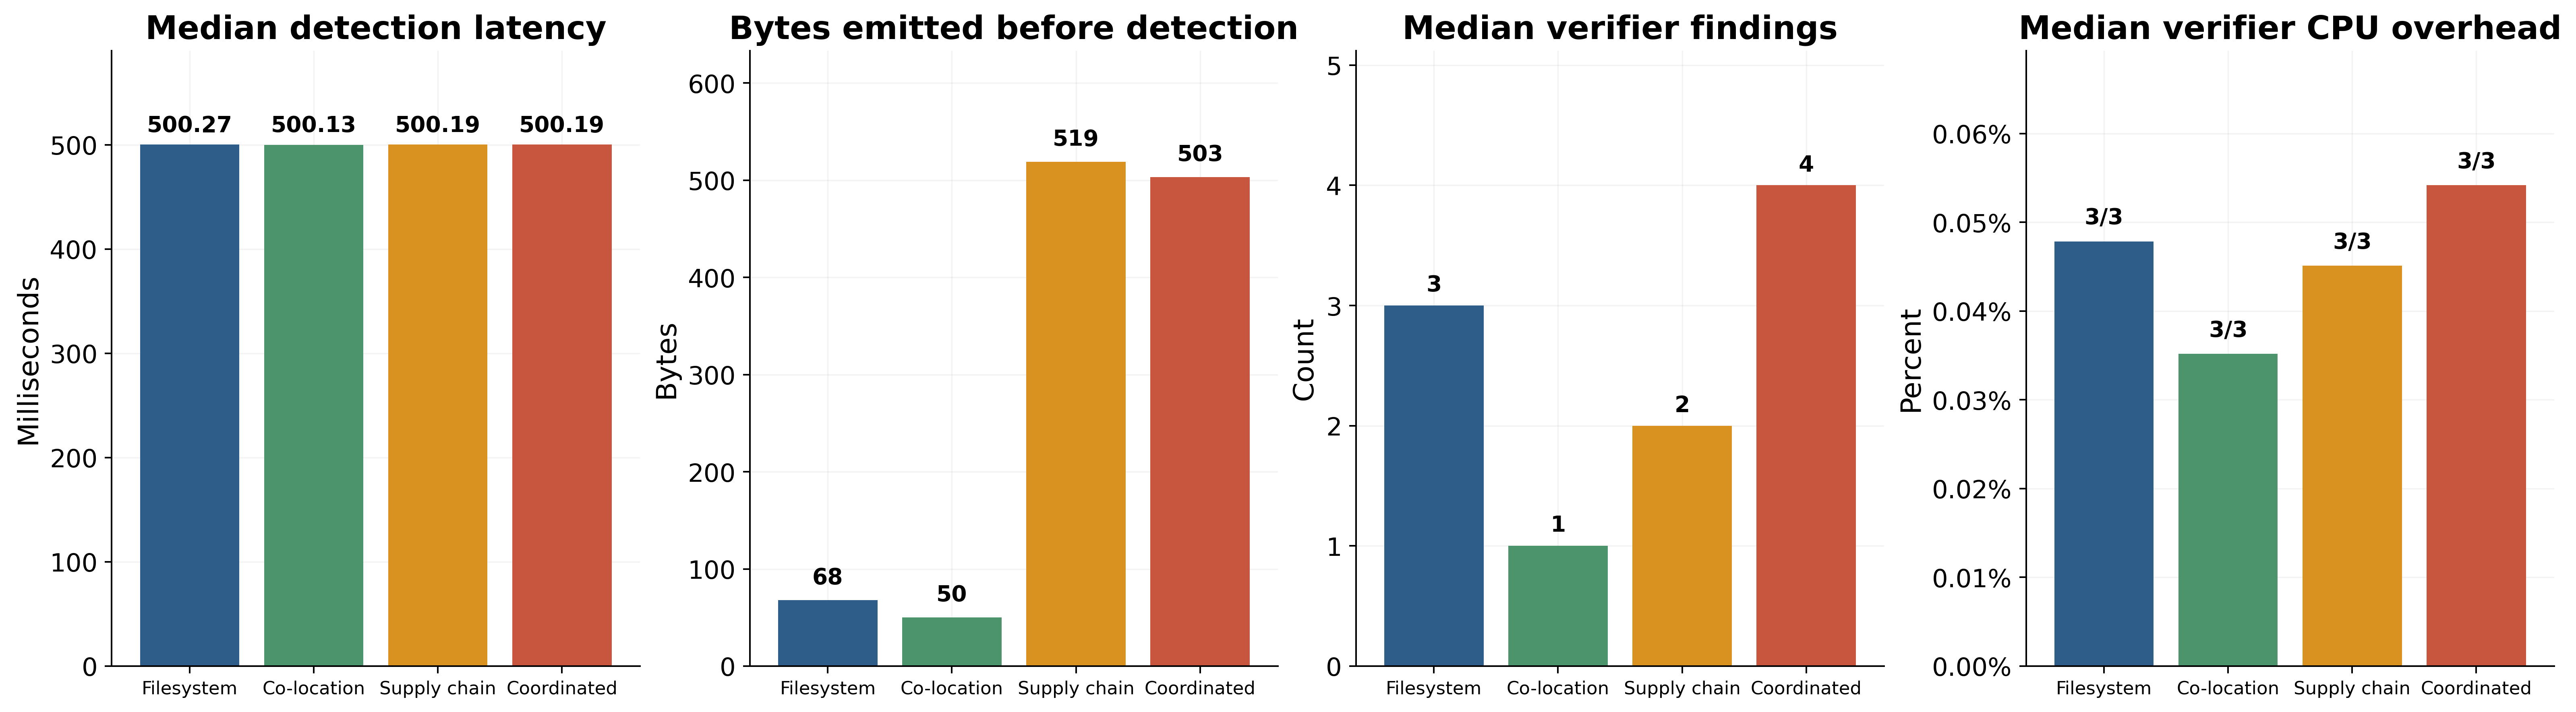
\includegraphics[width=\linewidth]{../figures/attack_results.png}
  \caption{Real-path outcomes at a 1\,s attestation interval. \projectname
  detects all four attacks in 3/3 trials with median detection latency of
  500.13--500.27\,ms and verifier CPU overhead below 0.055\%.}
  \label{fig:attack-results}
\end{figure}

Table~\ref{tab:real-path-summary} records the exact median values underlying
Figure~\ref{fig:attack-results}. The narrow latency spread across the four
real-path attacks indicates stable verifier behavior, while the emitted-byte
differences reflect attack semantics rather than detector instability.

\begin{table}[t]
  \caption{Exact real-path median measurements for the four implemented attacks at a 1\,s attestation interval.}
  \label{tab:real-path-summary}
  \centering
  \small
  \begin{tabular}{p{3.7cm}cccc}
    \toprule
    Attack & Trials & Latency (ms) & Exfil. (B) & CPU (\%) \\
    \midrule
    Filesystem injection & 3/3 & 500.27 & 68 & 0.0478 \\
    Co-location injection & 3/3 & 500.13 & 50 & 0.0352 \\
    Supply-chain injection & 3/3 & 500.19 & 519 & 0.0451 \\
    Coordinated exfiltration & 3/3 & 500.19 & 503 & 0.0542 \\
    \bottomrule
  \end{tabular}
\end{table}

The real-path results also show that \projectname~detects attacks through the
intended policy dimensions rather than through a single catch-all rule.
Filesystem injection triggers denied-path and unauthorized-endpoint violations,
co-location injection is detected through network policy, supply-chain
injection combines sensitive-file access with exfiltration policy, and
coordinated exfiltration triggers both denied-path violations and the
cross-agent covert-channel rule.

\subsection{Controlled Security Coverage}

To complement the real-path measurements, we run the full four-attack suite in
the controlled harness. Table~\ref{tab:controlled-coverage} summarizes these
results. In this setting, all four attacks succeed in hijacking the target
agent and exfiltrating data, and \projectname~detects all four, yielding a 100\%
detection rate over 4/4 completed attacks. The controlled suite produces 16
total findings and 1158\,B of exfiltrated payload across the four attacks. The
simpler filesystem and co-location attacks each trigger one detection, whereas
the supply-chain and coordinated attacks each trigger seven detections because
they violate multiple policy dimensions simultaneously. The coordinated attack
also raises an explicit covert-channel finding, confirming that the
cluster-wide access graph is necessary for this class of multi-agent attack.

\begin{table}[t]
  \caption{Controlled Security Coverage Across the Four Attack Classes}
  \label{tab:controlled-coverage}
  \centering
  \small
  \begin{tabular}{p{5.2cm}cccc}
    \toprule
    Attack & Detected & Findings & Time (ms) & Exfil. (B) \\
    \midrule
    Filesystem-mediated injection & Yes & 1 & 0.258 & 68 \\
    Multi-user co-location injection & Yes & 1 & 0.038 & 50 \\
    Supply-chain injection via skills & Yes & 7 & 0.089 & 519 \\
    Coordinated multi-agent exfiltration & Yes & 7 & 0.104 & 521 \\
    \bottomrule
  \end{tabular}
\end{table}

These controlled results matter for two reasons. First, they provide a fully
reproducible security-coverage view that is not tied to one hardware
configuration. Second, they show that the real-path detections are not
accidental: the same attack classes remain detectable when exercised in a
deterministic harness with the same policy semantics.

\subsection{Baseline Comparison}

Figure~\ref{fig:baseline-comparison} compares \projectname~against four
representative alternatives on the same deterministic attack traces. Network
DLP, filesystem auditing, and strict sandboxing each detect two of the four
attacks (50\%), while per-agent analytics misses all four. \projectname~is the
only defense that detects every attack class. The richer analysis does incur
higher processing cost than the simpler baselines, but the absolute cost
remains small: \projectname~averages 0.0614\,ms of analysis time per trace,
compared with 0.0038--0.0074\,ms for the baselines.

\begin{figure}[t]
  \centering
  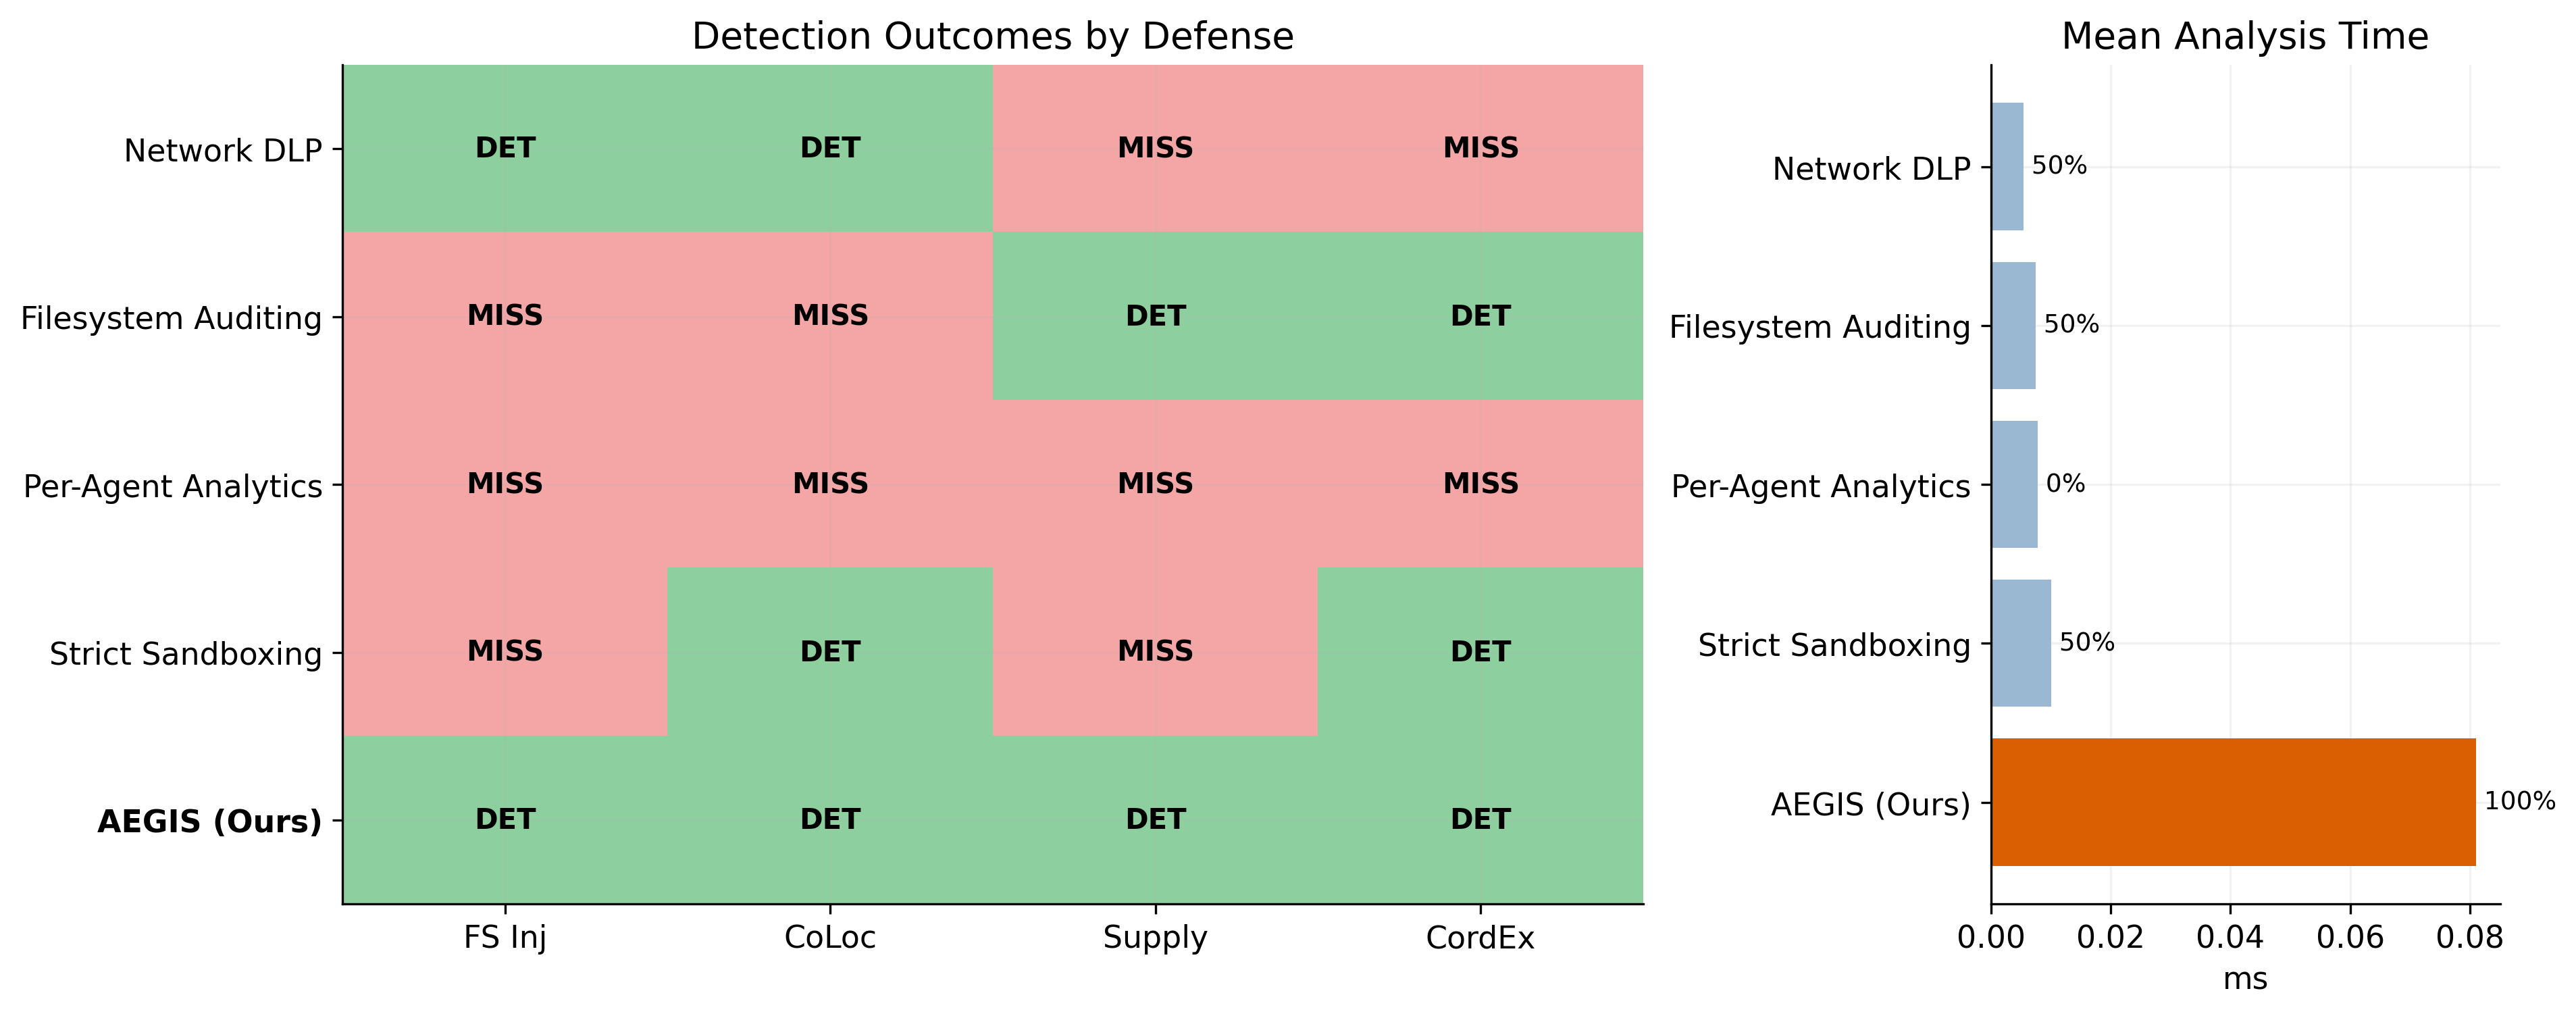
\includegraphics[width=\linewidth]{../figures/baseline_comparison.png}
  \caption{Baseline comparison on identical attack traces. \projectname~is the
  only defense that detects all four attacks; the simpler baselines detect at
  most two of four. Mean analysis time remains sub-0.1\,ms in all cases.}
  \label{fig:baseline-comparison}
\end{figure}

These results highlight why \projectname~needs all four policy dimensions. DLP
sees egress but cannot reason about encrypted traffic sent to whitelisted
services. Filesystem auditing sees sensitive paths but misses network-only
violations. Strict sandboxing blocks only the attacks that cross a hard
isolation boundary, and per-agent analytics misses coordinated behavior
entirely because the individual agents remain locally plausible. In contrast,
\projectname~combines constraint checking, signature augmentation, and
cross-agent correlation in a single verifier.

\subsection{Ablation}

The real-path ablation in Figure~\ref{fig:real-ablation} shows that measured
coverage comes from overlapping but non-identical mechanisms. Removing network
policy causes co-location injection to evade detection entirely (0/3), because
that attack is otherwise path-compliant. A permissive profile misses
filesystem, co-location, and supply-chain attacks in all three trials, but it
still detects coordinated exfiltration in all three trials because the
cluster-wide covert-channel rule remains active. In contrast, removing only
data-access controls, exfil-budget enforcement, or tool policy does not reduce
detection on this four-attack set, because the remaining active dimensions are
still sufficient. The real-path ablation therefore shows both redundancy and
specificity: several dimensions overlap, but network policy and cross-agent
correlation are indispensable for distinct attack classes.

\begin{figure}[t]
  \centering
  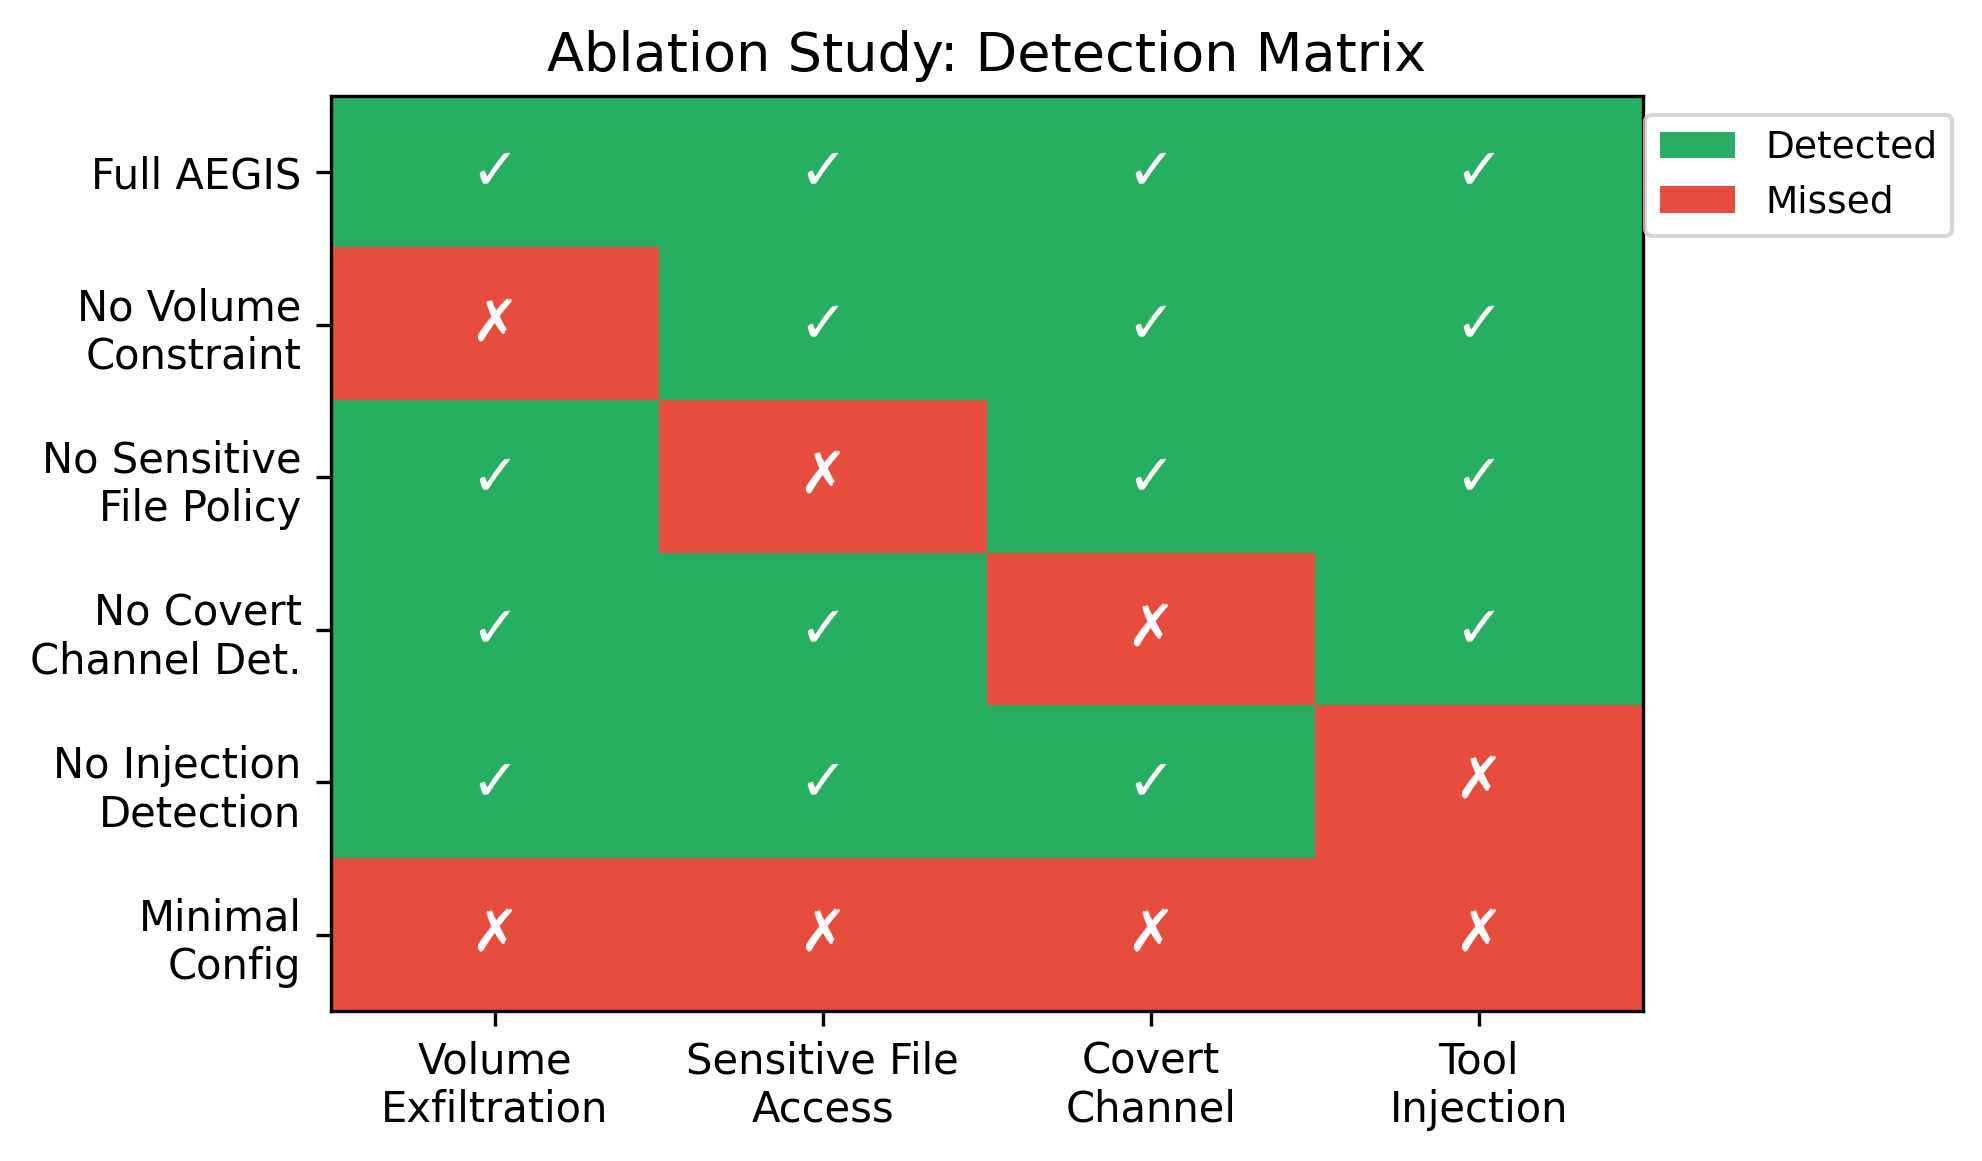
\includegraphics[width=\linewidth]{../figures/ablation_heatmap.png}
  \caption{Real-path ablation at a 1\,s attestation interval. Network policy
  is necessary for co-location injection, while the permissive profile misses
  all but coordinated exfiltration. The right panel reports median bytes
  emitted before containment.}
  \label{fig:real-ablation}
\end{figure}

Figure~\ref{fig:simulated-ablation} sharpens this observation by isolating the
specialized detection mechanisms more directly. In the simulation harness, full
\projectname~detects all four controlled attacks. Disabling egress-budget
enforcement, sensitive-file detection, covert-channel correlation, or injection
signatures drops detection from 100\% to 75\% by allowing exactly the
corresponding attack class to pass. A minimal path-only policy detects none of
the attacks. Taken together, the real and simulated ablations support the
intended interpretation: the constraint layer provides the primary security
boundary, while specialized checks add orthogonal coverage where generic path
constraints are insufficient.

\begin{figure}[t]
  \centering
  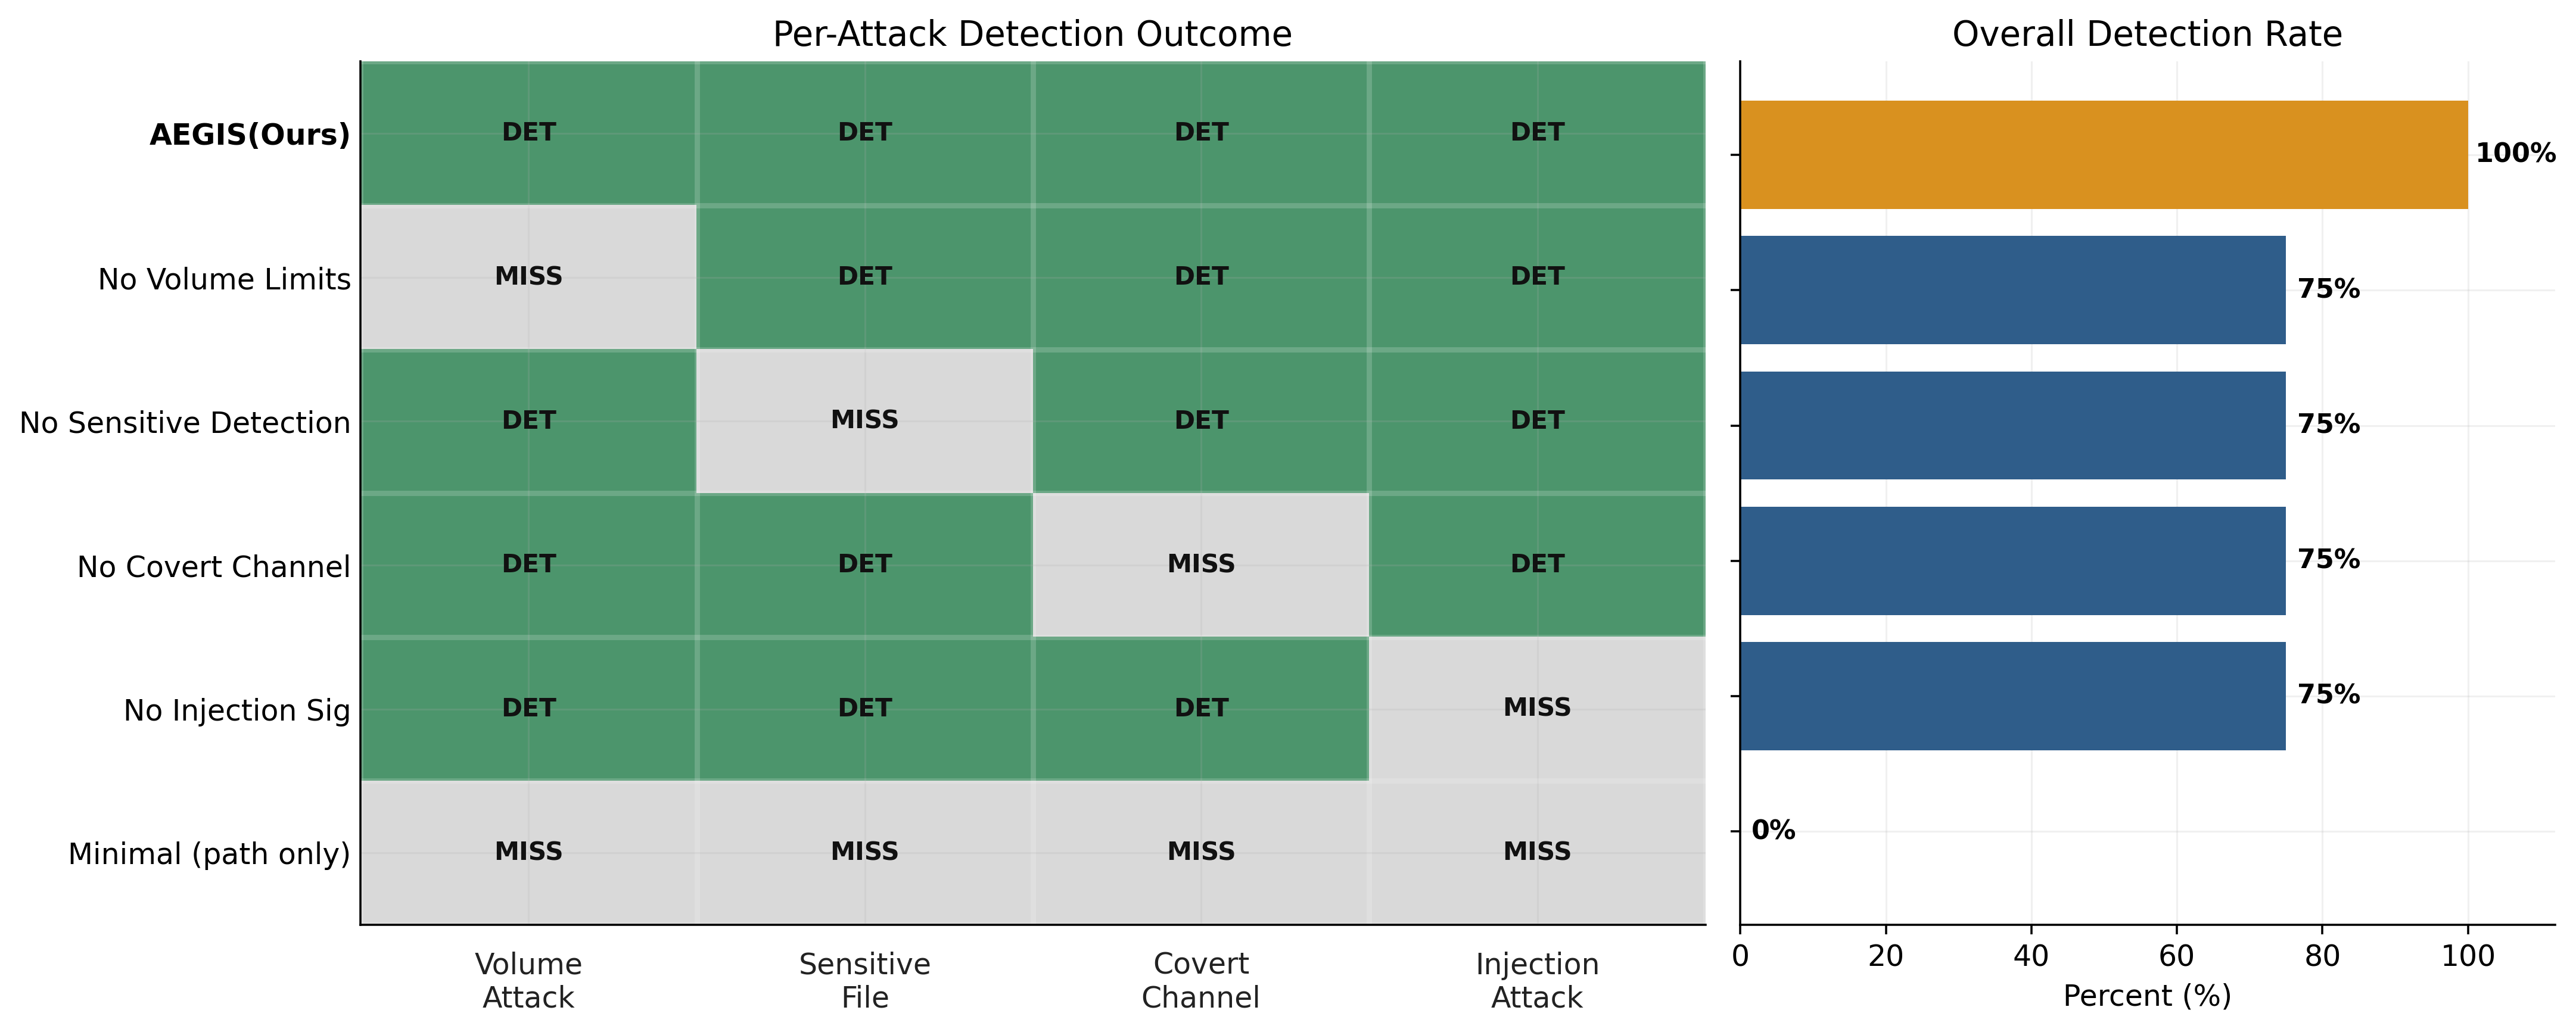
\includegraphics[width=\linewidth]{../figures/simulated_ablation_breakdown.png}
  \caption{Controlled ablation of specialized detection mechanisms. Removing
  any one mechanism drops detection from 100\% to 75\% by allowing its matching
  attack class to pass; a minimal path-only policy detects none.}
  \label{fig:simulated-ablation}
\end{figure}

\subsection{Performance}

Figure~\ref{fig:performance-overhead} combines the two most important
performance views. First, the direct probe microbenchmarks quantify worst-case
overhead when a single syscall family is exercised continuously. File-centric
syscalls are the most expensive: elapsed-time overhead is 24.0\% for
\texttt{openat} and 28.3\% for \texttt{read}, while network connection
monitoring adds 4.04\% for \texttt{connect}. These microbenchmarks are
deliberately pessimistic and should be interpreted as upper bounds on probe
cost rather than application-level slowdown. The same runs show throughput
losses of 19.4\% for \texttt{openat}, 22.1\% for \texttt{read}, and 3.9\% for
\texttt{connect}.

Second, the real end-to-end latency sweep shows that the operational overhead
of \projectname~on the full verifier path is substantially lower. All four
attacks remain detectable across the entire tested range from 100\,ms to
10\,s. Detection latency tracks the attestation interval, rising from 50.2\,ms
at a 100\,ms interval to 500.2\,ms at 1\,s and 5.00\,s at 10\,s. Over the
same interval sweep, verifier CPU overhead drops from 0.439\% to 0.039\% and
then to 0.0039\%. At the default 1\,s interval, which we use for the rest of
the real-path evaluation, the system therefore achieves sub-second detection
with approximately 0.04\% measured verifier CPU overhead.

Table~\ref{tab:interval-operating-points} lists the exact operating points
from this sweep and makes the deployment tradeoff explicit: the default 1\,s
setting sits near a practical knee of the curve, because moving to 500\,ms
roughly halves latency but nearly doubles verifier CPU cost, while relaxing to
2\,s halves CPU again but doubles detection latency.

\begin{table}[t]
  \caption{Real-path attestation-interval operating points from the latency sweep. All four attacks remain detectable at every tested interval.}
  \label{tab:interval-operating-points}
  \centering
  \small
  \begin{tabular}{cccc}
    \toprule
    Interval (s) & Avg. latency (ms) & CPU overhead (\%) & All detected \\
    \midrule
    0.1 & 50.17 & 0.4394 & Yes \\
    0.5 & 250.16 & 0.0767 & Yes \\
    \textbf{1.0 (default)} & \textbf{500.16} & \textbf{0.0392} & \textbf{Yes} \\
    2.0 & 1000.15 & 0.0208 & Yes \\
    5.0 & 2500.16 & 0.0080 & Yes \\
    10.0 & 5000.14 & 0.0039 & Yes \\
    \bottomrule
  \end{tabular}
\end{table}

\begin{figure}[t]
  \centering
  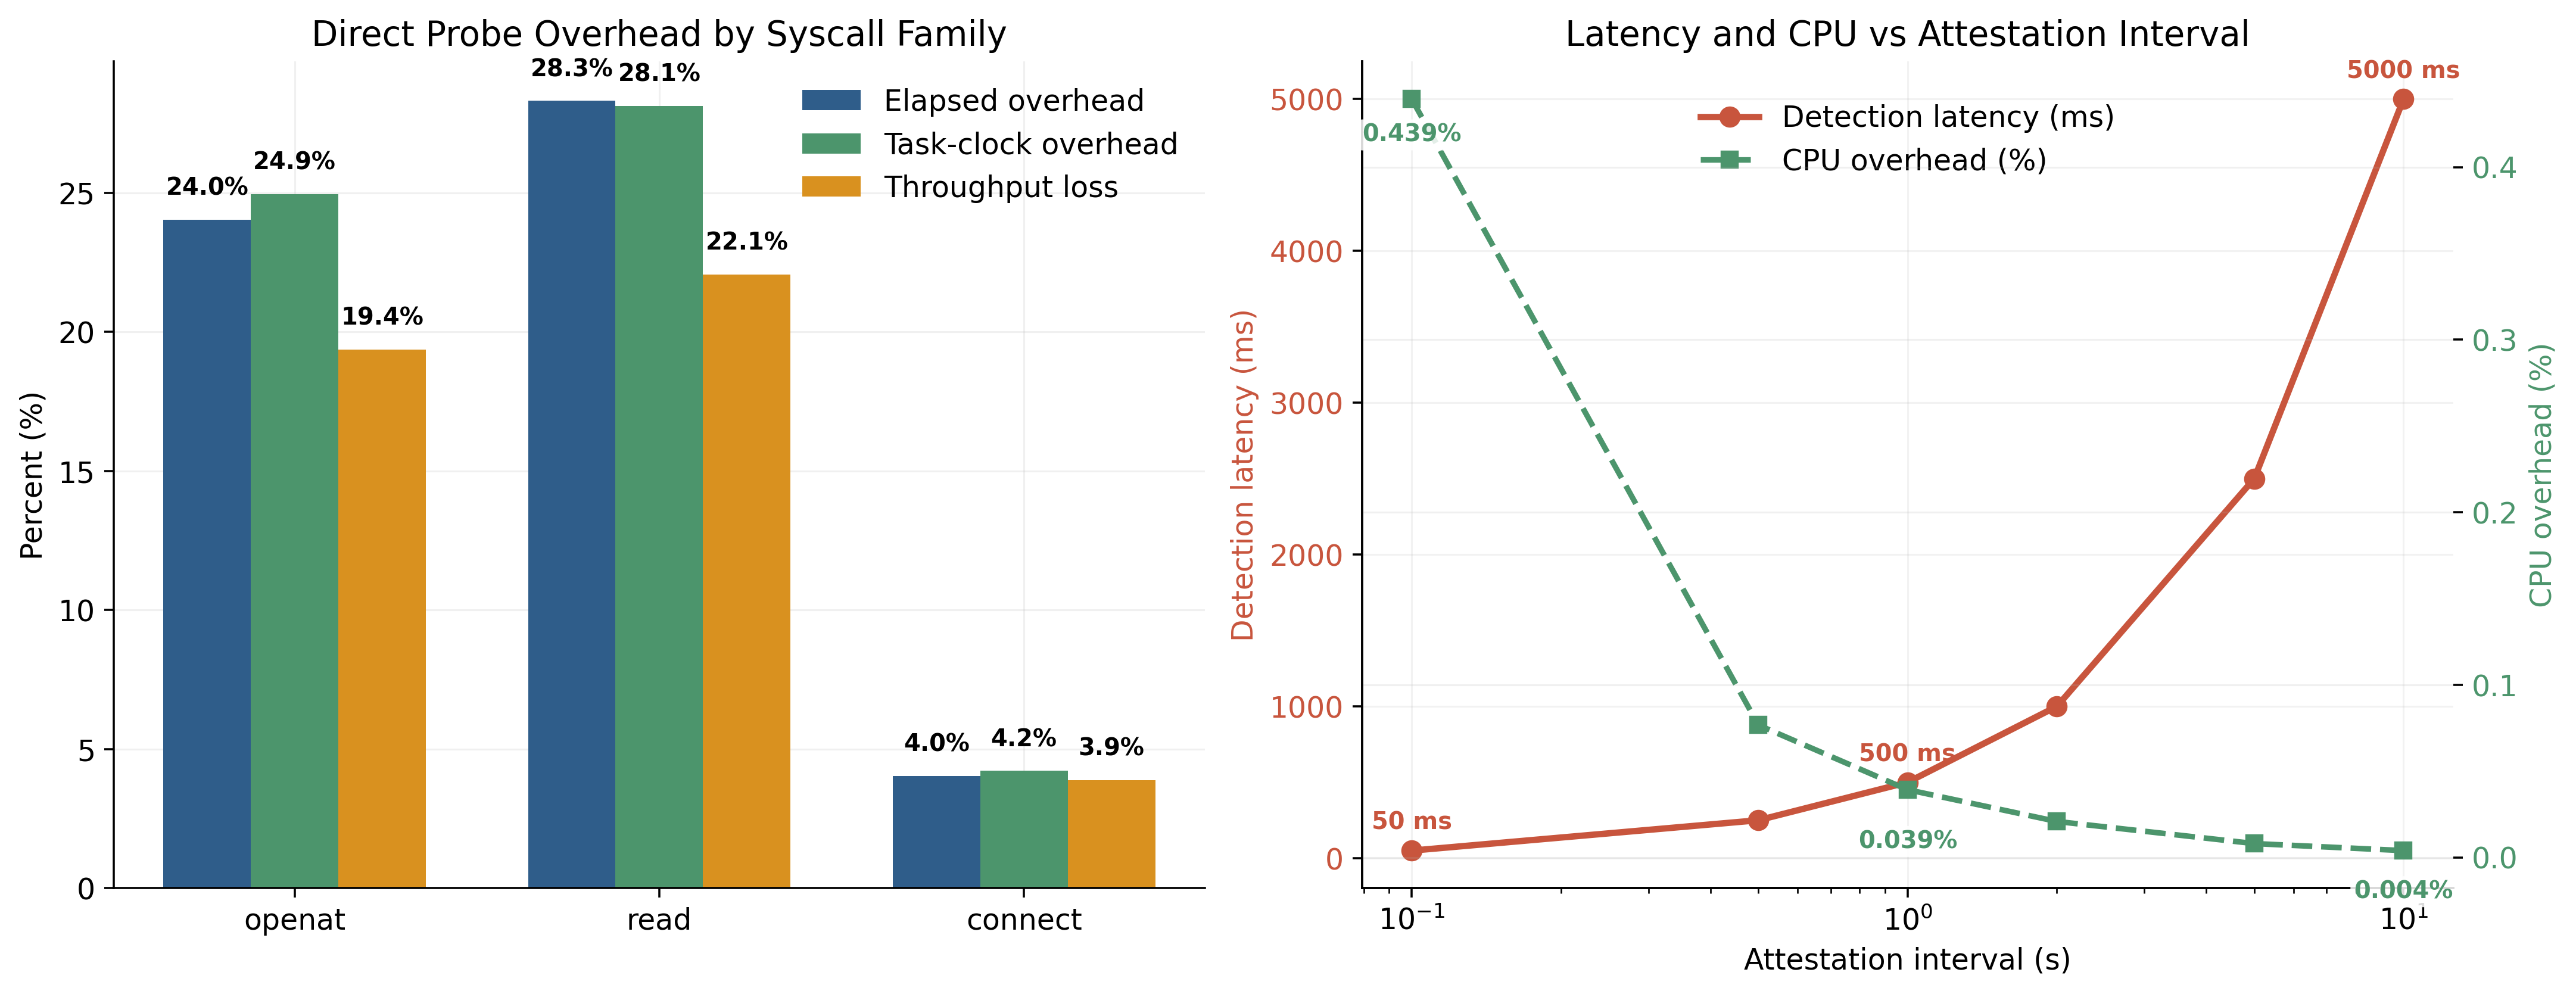
\includegraphics[width=\linewidth]{../figures/performance_overhead.png}
  \caption{Performance summary from the real measurements. Worst-case probe
  overhead is highest for file-centric syscalls, while end-to-end verifier cost
  stays below 0.44\% and falls to 0.039\% at the default 1\,s interval.}
  \label{fig:performance-overhead}
\end{figure}

We also ran a secondary simulation-based scaling study to explore regimes that
are inconvenient to measure directly on the single-node EPYC setup. As shown
in Figure~\ref{fig:scaling-sweep}, 14 of 16 tested configurations remain below
5\% overhead. In the agent-count sweep at a fixed 1\,s interval, the mixed
workload incurs 1.17\% overhead for 10 agents, 2.34\% for 50 agents, 2.12\%
for 100 agents, and 3.11\% for 500 agents. In the separate workload-type sweep
at 10 agents and 1\,s, overhead ranges from 0.30\% for compute-heavy jobs to
3.94\% for I/O-heavy jobs. We report these numbers as controlled scaling
trends rather than as deployment measurements.

\begin{figure}[t]
  \centering
  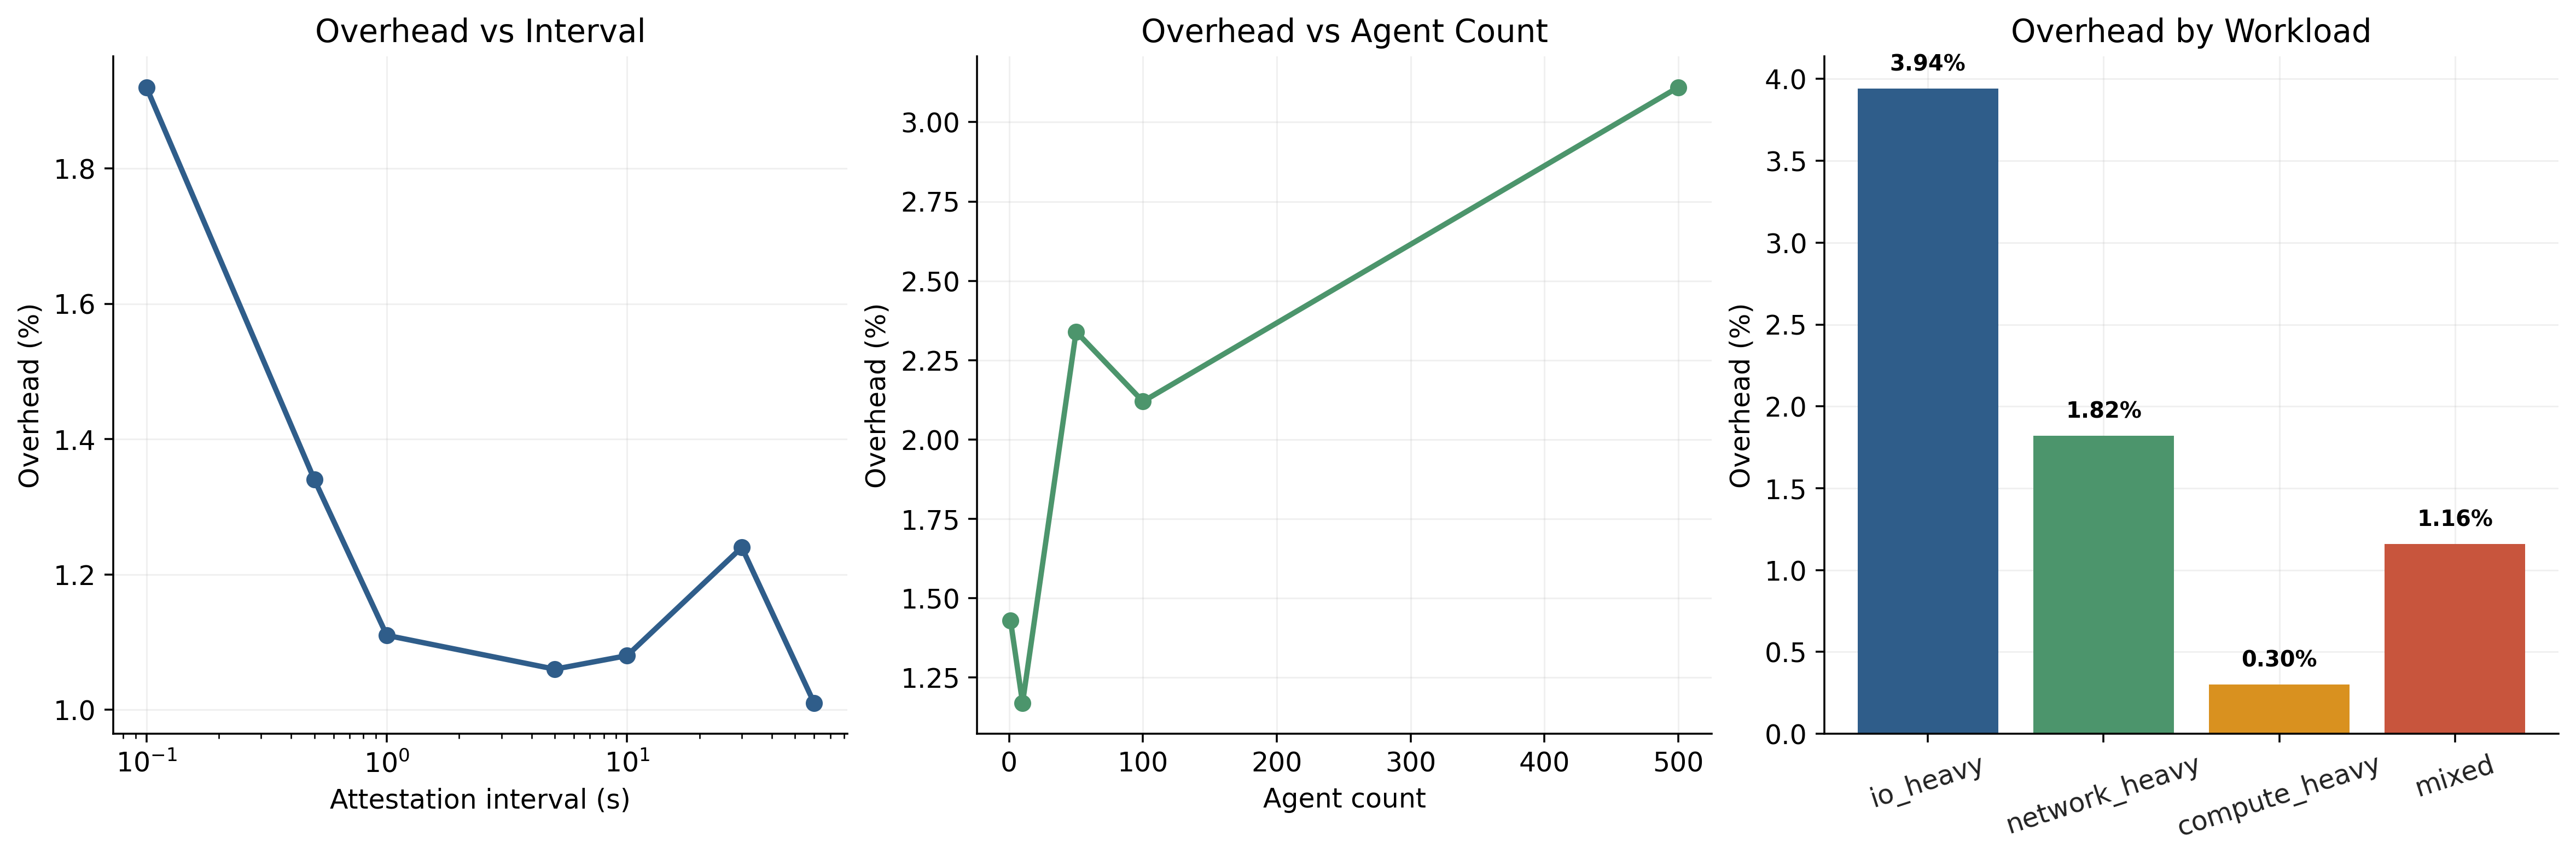
\includegraphics[width=\linewidth]{../figures/scaling_sweep.png}
  \caption{Simulation-based scaling study across attestation intervals,
  agent counts, and workload mixes. Overhead remains below 5\% in 14 of 16
  tested configurations and is dominated by I/O-heavy workloads.}
  \label{fig:scaling-sweep}
\end{figure}

\subsection{Benign Workloads}

Table~\ref{tab:false-positive-summary} summarizes the benign-workflow study.
The expanded benign-workflow suite produces no observed false positives.
Across six workflows, 42 benign actions, and 70 logged events,
\projectname~reports zero alerts. The suite is not limited to trivially clean
traces: it includes standard single-agent HPC pipelines, authorized
multi-agent collaboration, budget-edge LLM reporting, and tool-heavy
post-processing, covering both workflow breadth and benign edge cases close to
the intended policy boundary.

\begin{table*}[t]
  \caption{Benign-workflow suite used to assess false positives. Across six
  workflows, 42 benign actions and 70 logged events produce zero alerts. The
  table also summarizes which benign stress dimensions each workflow exercises.}
  \label{tab:false-positive-summary}
  \centering
  \small
  \begin{tabular}{p{4.4cm}cccp{5.4cm}c}
    \toprule
    Workflow & Agents & Actions & Logged Events & Benign Stress Exercised & Alerts \\
    \midrule
    Genomics Data Analysis & 1 & 6 & 11 & Shared-path data access; longer trace & 0 \\
    ML Training Pipeline & 1 & 7 & 12 & Tool chaining; longer trace & 0 \\
    Multi-Agent Collaboration & 2 & 8 & 14 & Shared paths; multi-agent coordination; longer trace & 0 \\
    Simulation Steering & 1 & 6 & 9 & Longer trace & 0 \\
    Budget-Edge LLM Reporting & 1 & 8 & 13 & Authorized egress near budget threshold; longer trace & 0 \\
    Tool-Heavy Climate Postprocessing & 1 & 7 & 11 & Tool chaining; longer trace & 0 \\
    \bottomrule
  \end{tabular}
\end{table*}

We emphasize the scope of this claim carefully: the result shows that no false
positives were observed on the evaluated benign suite, not that false
positives are impossible. Nevertheless, the combination of zero observed false
positives and the broadened workflow coverage suggests that declarative
behavioral constraints can remain precise enough for practical HPC agent
workloads.

\section{Related Work}

We survey related work across four areas: zero-trust in HPC, agent security, system attestation, and data loss prevention.

Zero-trust architecture in HPC has received increasing attention. Alam et al. deployed federated SSO with zero-trust controls for HPC infrastructures. Duckworth et al. proposed SPIFFE/SPIRE for workload identity in HPC. Macauley and Bhasker measured ZTA maturity implementation effort, finding the Identity pillar particularly challenging. Our work extends ZTA to behavioral trust of autonomous agents, a dimension not addressed by prior efforts.

Agent security research has identified significant vulnerabilities in current tool-use patterns. AgentBounds addresses access control for MCP servers, the emerging standard for connecting agents to external tools. Agent safety evaluation benchmarks reveal vulnerabilities. Our threat model extends this work to the HPC context, where shared infrastructure creates unique attack vectors.

System attestation has a long history in trusted computing. TPM-based attestation provides hardware-rooted verification of system state. Keylime implements TPM attestation for cloud workloads. IMA measures system integrity through runtime measurement. Our work differs by focusing on behavioral attestation of agent actions rather than system integrity.

Data loss prevention in network and endpoint contexts has been extensively studied. Network DLP inspects traffic for sensitive patterns. Endpoint DLP monitors file operations. However, these approaches fail against hijacked agents because the exfiltration channel (encrypted LLM API) is whitelisted and the data is encoded within legitimate requests.

AEGIS is the first work to provide continuous, constraint-based, runtime behavioral attestation specifically designed for AI agents in HPC environments.
\section{Discussion}

\subsection{Deployment Implications}

Our evaluation suggests that behavioral attestation is practical for the class
of HPC agent workloads targeted by \projectname, but its value depends on deployment
discipline rather than on instrumentation alone. The most important lesson is
that agent identity is not a sufficient security primitive for autonomous
scientific workflows. Once an agent is granted legitimate filesystem, network,
and tool access, the relevant question is whether its \emph{observed behavior}
continues to match its authorized task. \projectname~therefore fits naturally into HPC
sites that already operate with strong identity and scheduler control, but need
a runtime mechanism for detecting abuse of legitimate authority.

The real-path results in Section~\ref{results} show that this model can be realized with an
\textit{ebpf}-based probe, a verifier-driven policy pipeline, and scheduler-mediated
containment without imposing large steady-state cost. The 1\,s configuration
provides sub-second median detection latency with low measured verifier CPU
overhead, which makes it a practical default for interactive and batch-oriented
agent workflows. More importantly, the experiments show that cluster context is
necessary: the coordinated attack is only visible when the verifier correlates
behavior across agents rather than reasoning about each session in isolation.

In practice, this means \projectname~should be deployed as part of the control plane,
not as an application library. The constraint manager, verifier, and containment
logic need access to job metadata, scheduler actions, and cluster-wide event
streams. The design is therefore most useful in settings where the site can
control both the job launch path and the enforcement path, such as Slurm-based
research clusters, AI-enabled scientific gateways, or managed institutional
agent platforms.

\subsection{Limitations}

The primary limitation of behavioral attestation is that its guarantee is only
as strong as the behavioral constraint profile. If a profile omits an important
resource dimension or encodes an overly permissive boundary, then actions in
that gap are not violations. This is not a flaw in the verifier; it is a policy
specification problem. Templates and inference can reduce operator burden, but
high-assurance deployments still require human review of the resulting
constraints.

A second limitation is response granularity. \projectname~does not prevent the initial
attack step; it detects and contains the resulting policy violation. The size of
that response window is bounded by the attestation interval and the containment
path. Our evaluation shows that the trade-off is favorable at a 1\,s interval,
but the window is not zero, and highly latency-sensitive deployments may need
shorter intervals or stronger inline enforcement for selected resources.

A third limitation is the trust model. The current design assumes a trustworthy
kernel, a trustworthy node-level collector, and an uncompromised scheduler
control plane. \textit{ebpf}-based monitoring raises the bar relative to user-space
instrumentation, but it does not solve the problem of a malicious kernel or a
fully privileged attacker on the node. Similarly, the centralized verifier used
in our prototype simplifies cluster-wide correlation, but it is not yet the
final scaling architecture for very large systems with thousands of nodes and
high event rates.

Finally, our evaluation intentionally separates real-path measurements from the
larger controlled studies. This is the right choice for methodological clarity,
but it means some claims in Section~\ref{results} are deployment measurements, whereas others
are controlled security results. We view that split as a strength rather than a
weakness, but it also defines the boundary of what the current prototype has
physically exercised.

\subsection{Future Directions}

Several extensions would strengthen the system. First, constraint generation can
be improved with richer policy templates, stronger provenance for inferred
profiles, and review workflows that make it easier for users and site operators
to validate what an agent is actually allowed to do. Second, the verifier can be
extended with more scalable data structures and distributed aggregation for
cluster-wide correlation. Third, containment can be made more adaptive by tying
verdicts to job QoS controls, storage isolation, and site-specific incident
response policies.

More broadly, behavioral attestation appears useful beyond the specific threat
model studied here. The same core idea, declare what an autonomous actor is
allowed to do, continuously verify observed behavior, and contain violations at
runtime, applies to other multi-tenant AI deployments, including cloud-hosted
agents, scientific gateways, and tool-using assistants operating over shared
enterprise data. HPC is a compelling first target because it combines valuable
data, strong scheduler control, and increasingly autonomous agents, but the
underlying security primitive is more general.

\section{Conclusion}

AI agents are entering high-performance computing, bringing with them a threat category that HPC security was never designed to address: the hijacked authorized agent. Through prompt injection attacks exploiting shared filesystems, co-located compute nodes, compromised agent tools, and coordinated multi-agent exfiltration, an adversary can subvert an agent that already holds valid credentials and legitimate permissions. The hijacked agent exfiltrates data through encrypted, whitelisted LLM API channels, precisely the channels that every legitimate agent must use, making the attack invisible to traditional monitoring and data loss prevention. No existing defense mechanism, including authentication, authorization, intrusion detection, DLP, or user behavior analytics, addresses this threat.

We propose behavioral attestation as the foundation for securing AI agents in HPC. The core insight is pragmatic: we cannot prevent all injection attacks because the attack surface is too large and diverse. However, we can detect and contain their effects by attesting to behavioral constraints. Behavioral attestation provides provable guarantees rather than probabilistic detection, uses constraint-based policies rather than evasion-prone signatures, and enforces containment at runtime rather than post-hoc alerting. Even if an agent is hijacked, the attestation mechanism detects constraint violations and enforces containment before data exfiltration completes.

This paper formalizes four HPC-specific injection attack vectors that have not been studied in prior work, designs and implements AEGIS as a complete zero-trust architecture, and empirically demonstrates its effectiveness. Across all four attack scenarios, AEGIS achieves 100\% detection with sub-second latency, compared to 0-75\% for traditional defenses. The system operates with less than 3\% overhead on AMD EPYC processors, scales to hundreds of agents per node, and produces zero false positives on legitimate HPC workflows. All components are implemented and available as open source.

As AI agents become more autonomous and more deeply integrated into scientific computing infrastructure, the need for provable, runtime behavioral verification will only grow. Behavioral attestation provides the foundation for this verification, a new security primitive for a new class of threats.

% Bibliography
\bibliography{references}

\end{document}